\section{Manual de Usuario}
En este capítulo vamos a explicar como usar el software en cada uno de sus apartados.

\newpage

\subsection{Inicio de Sesión}
Para acceder a la aplicación, necesitamos pasar si o si por la pantalla de login. Esta pantalla es la primera que se ve en el primer acceso a la aplicación.

Para poder probar dicha aplicación de forma rápida, aconsejamos usar el usuario por defecto.
\begin{itemize}
    \item Username: \textbf{test}
    \item Password: \textbf{test}
\end{itemize}

\begin{figure}[H]
    \centering
    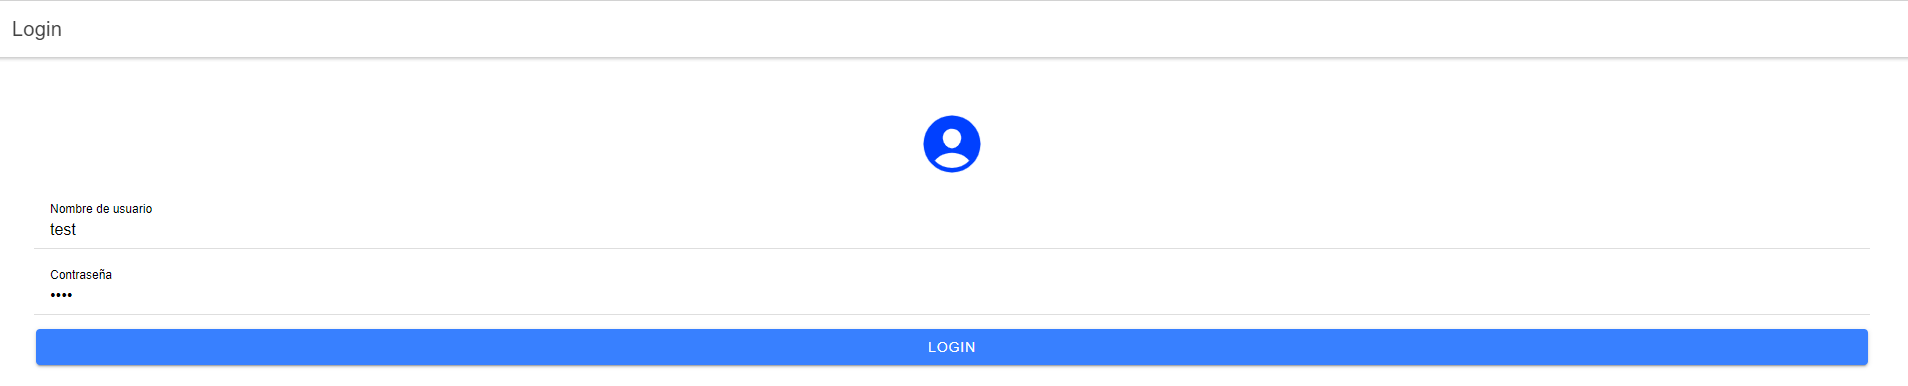
\includegraphics[width=1\linewidth]{images/user-manual/login.png}
    \caption{Inicio de Sesión}
\end{figure}

\subsection{Cerrar Sesión}
Para poder cerrar sesión, previamente se tiene que estar logeado y en el menú del dashboard. Una vez que se cumplen estas condiciones, es tan fácil como pulsar en la opción con el texto ``Cerrar sesión''.

\begin{figure}[H]
    \centering
    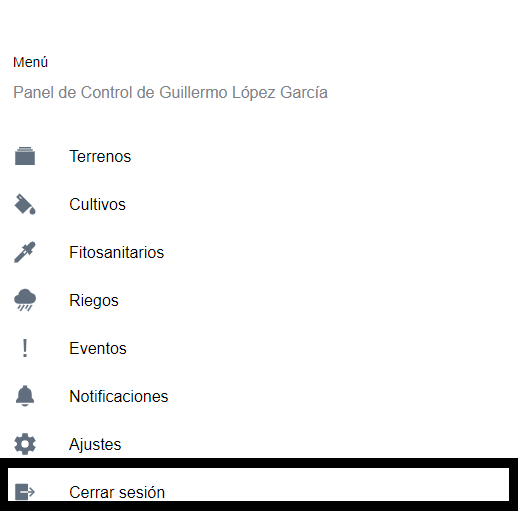
\includegraphics[width=0.7\linewidth]{images/user-manual/logout.png}
    \caption{Cerrar Sesión}
\end{figure}

\subsection{Dashboard}
Esta es la pantalla principal que ve el usuario cuando pasa el login. En esta pantalla, se puede ver el menú y todas las opciones que este tiene.

\begin{figure}[H]
    \centering
    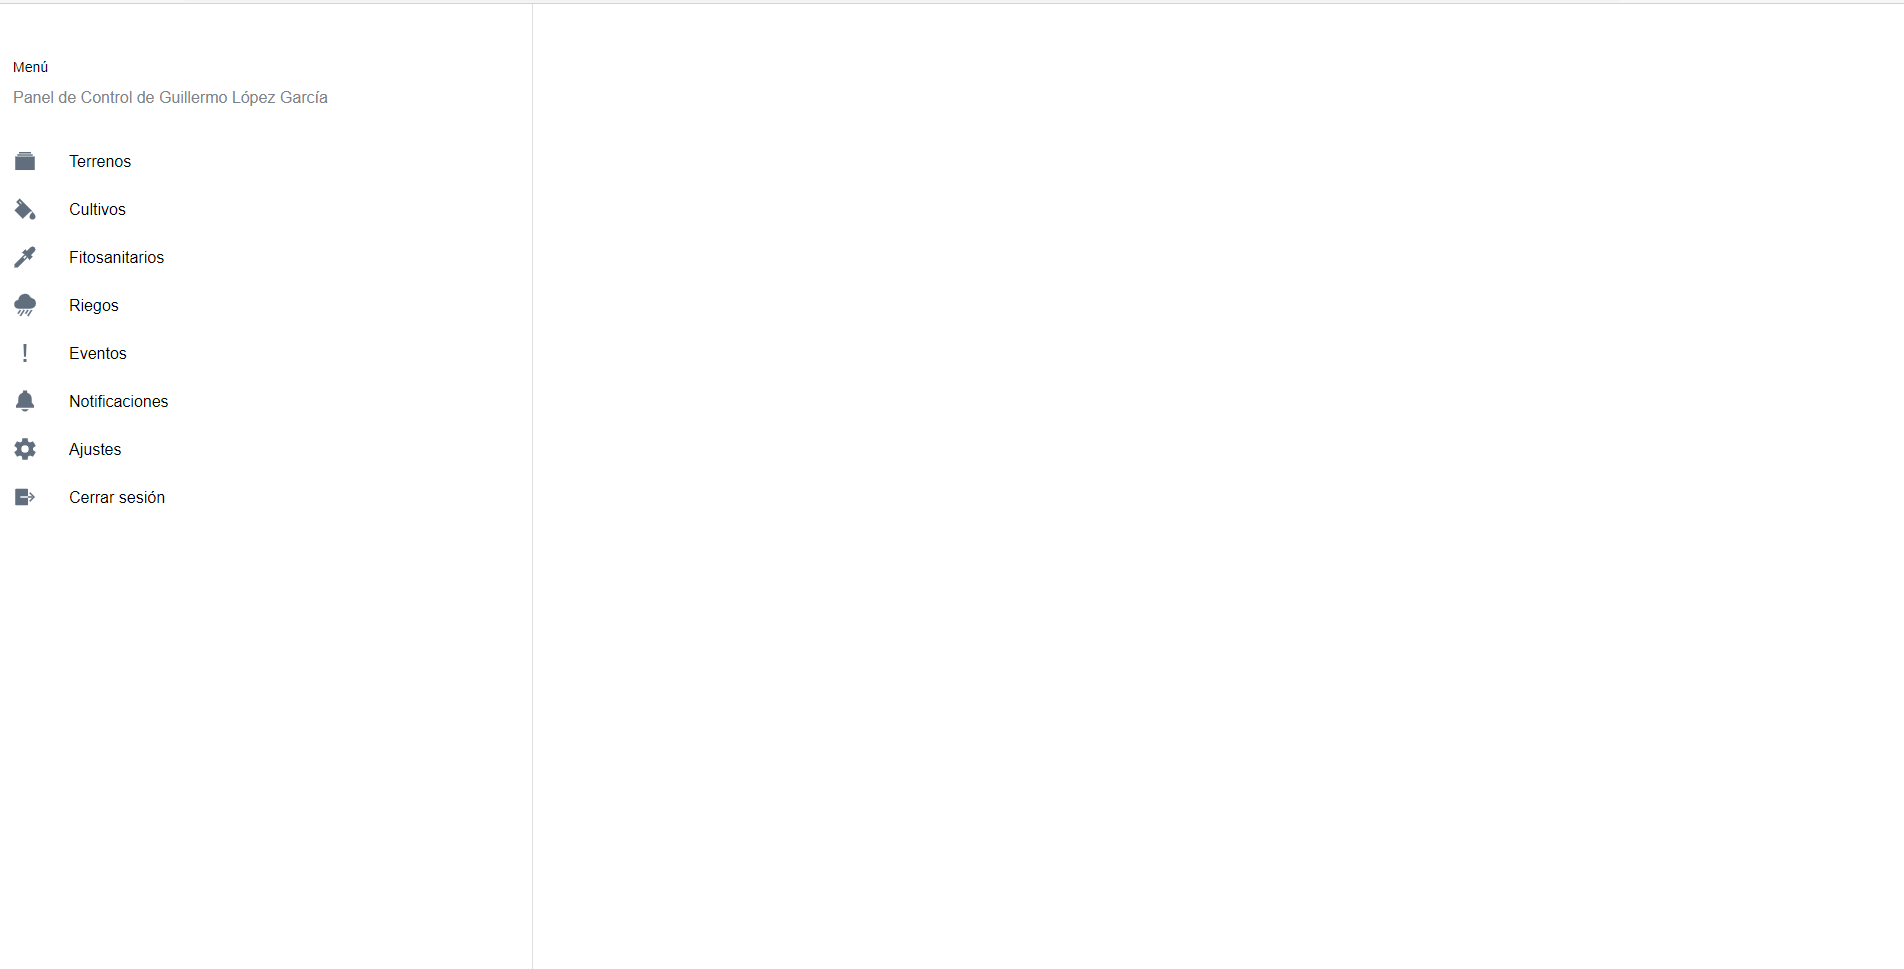
\includegraphics[width=0.7\linewidth]{images/user-manual/dashboard.png}
    \caption{Dashboard}
\end{figure}

\subsection{Inicio}
Esta pantalla, se convierte en la principal en caso de que se este usando la aplicación móvil o se este accediendo a la web desde un móvil.

Desde esta pantalla, se puede acceder a cualquiera de las secciones de la aplicación.

\begin{figure}[H]
    \centering
    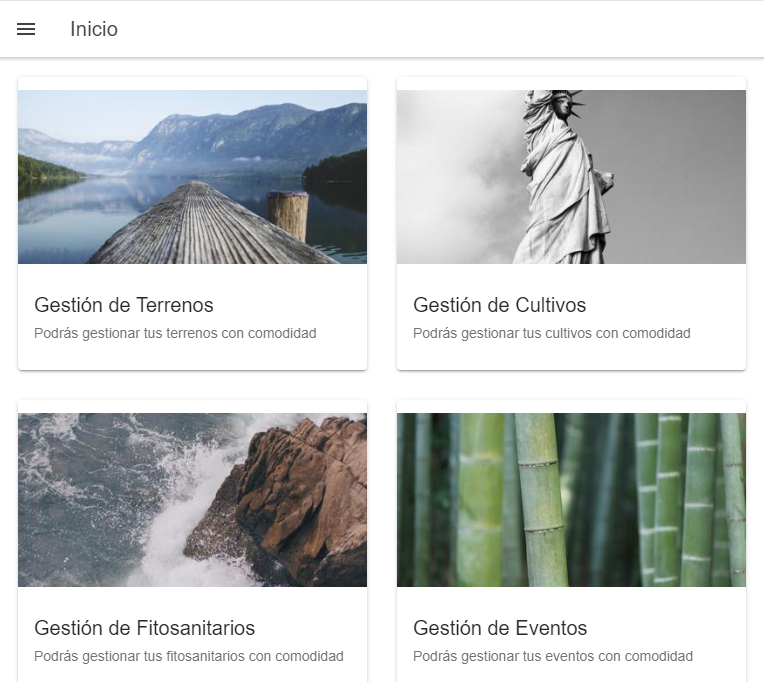
\includegraphics[width=0.7\linewidth]{images/user-manual/inicio.png}
    \caption{Inicio}
\end{figure}

\subsection{Terrenos}
En esta sección, se permite todo el CRUD de los terrenos. A continuación, se explica como se hace cada una de las operaciones.

\subsubsection{Listar}
Para listar los terrenos disponibles, tan solo tendremos que entrar en la sección de terrenos y de entrada los listará a todos, como se puede apreciar en la Figura 9.5.
\begin{figure}[H]
    \centering
    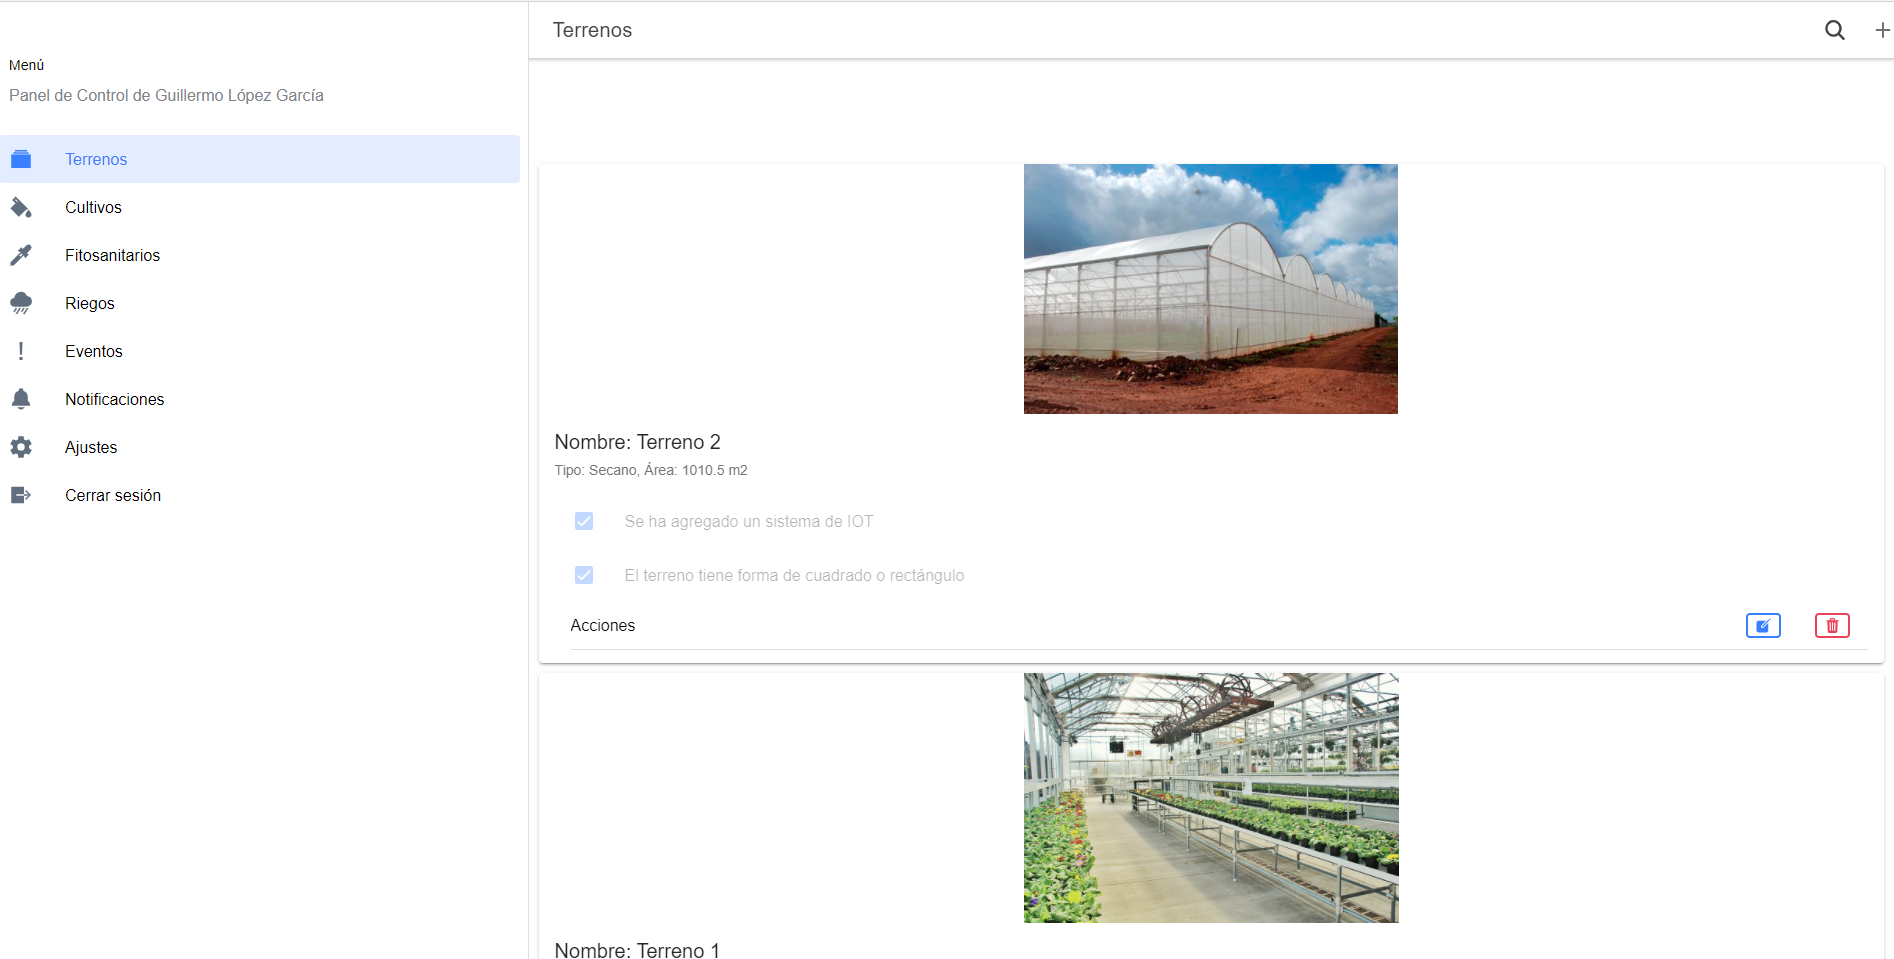
\includegraphics[width=0.7\linewidth]{images/user-manual/farmableland/list.png}
    \caption{Listar Terrenos}
\end{figure}

\subsubsection{Buscar}
Para buscar un terreno, el usuario debe pulsar en la barra superior que existe en la sección de terrenos y escribir la búsqueda deseada. A continuación, se volverá a listar los terrenos pero con el filtro aplicado, como se puede apreciar en la Figura 9.6.
\begin{figure}[H]
    \centering
    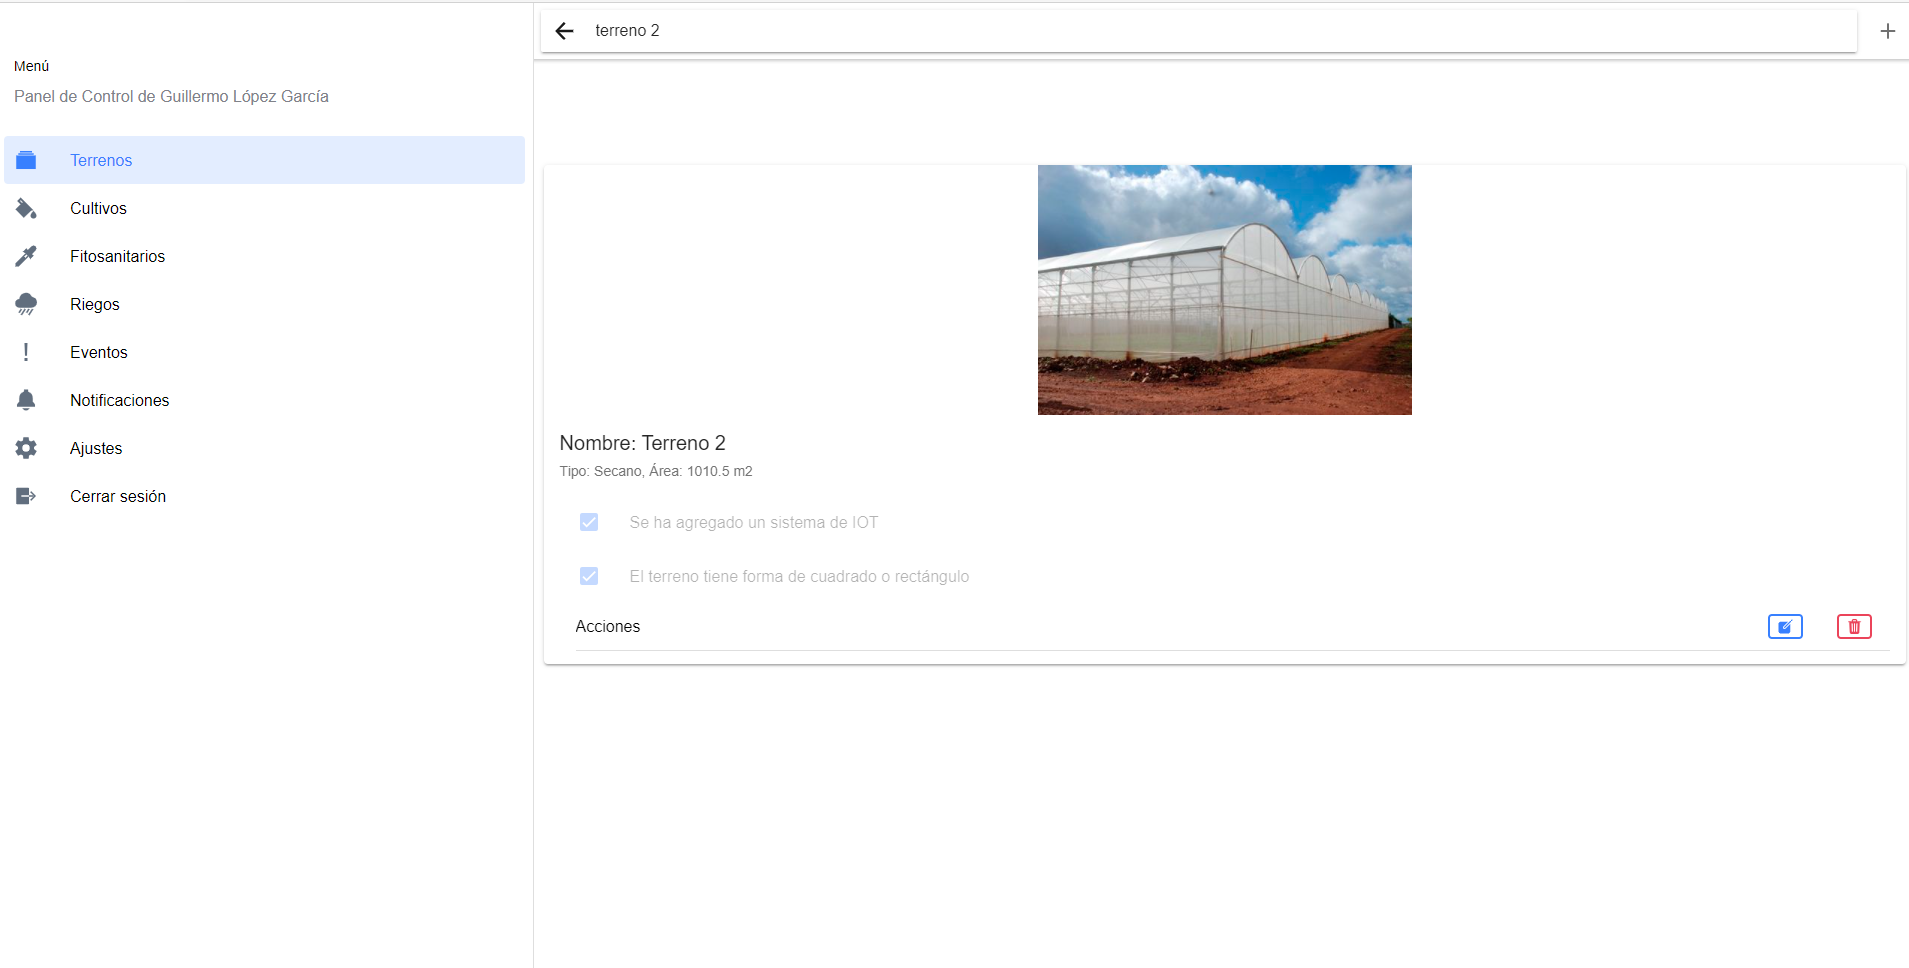
\includegraphics[width=0.7\linewidth]{images/user-manual/farmableland/search.png}
    \caption{Buscar Terrenos}
\end{figure}

\subsubsection{Añadir}
Para añadir un terreno, el usuario debe pulsar en el icono con el símbolo ``+'' y le llevará al formulario, que aparece en la Figura 9.7, para añadir un terreno. Una vez que el usuario lo rellene de forma correcta, se creará el terreno correspondiente.
\begin{figure}[H]
    \centering
    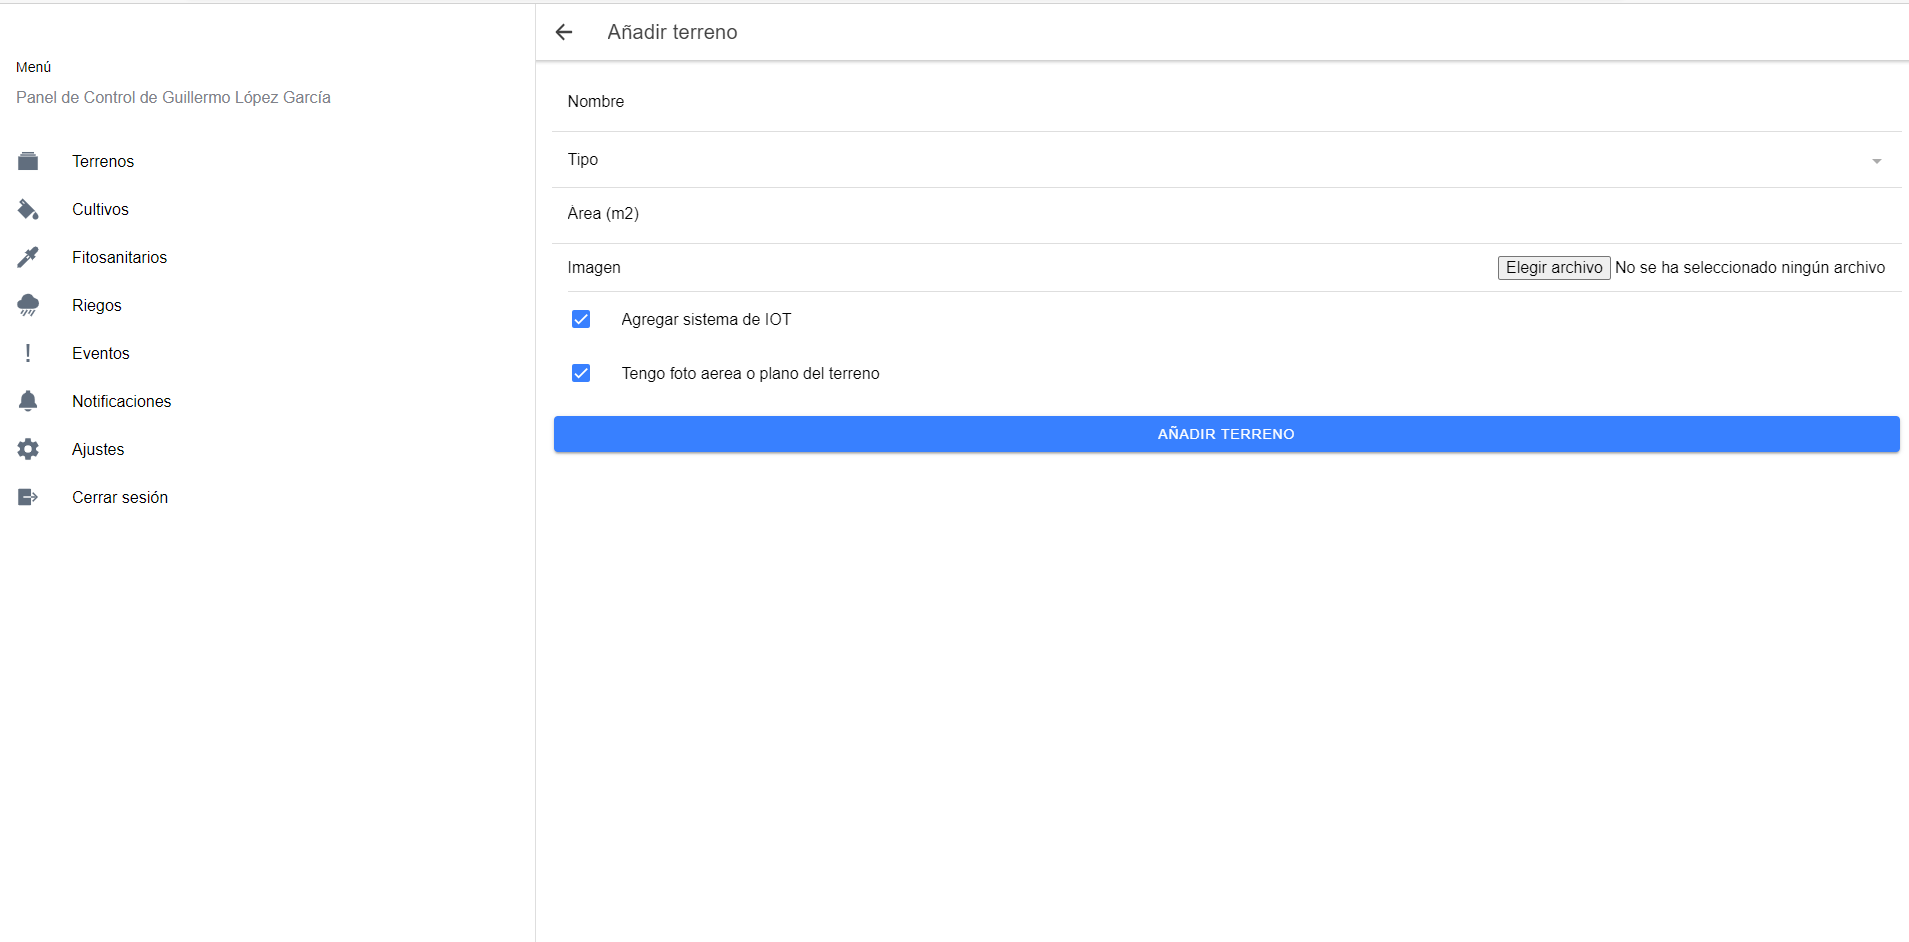
\includegraphics[width=0.7\linewidth]{images/user-manual/farmableland/create.png}
    \caption{Añadir Terreno}
\end{figure}

\subsubsection{Modificar}
Para modificar un terreno, el usuario debe pulsar en icono de editar del terreno y lo llevará al formulario que se puede apreciar en la Figura 9.8. Una vez cambie los valores y además dichos valores sean correctos, el terreno se actualizará.
\begin{figure}[H]
    \centering
    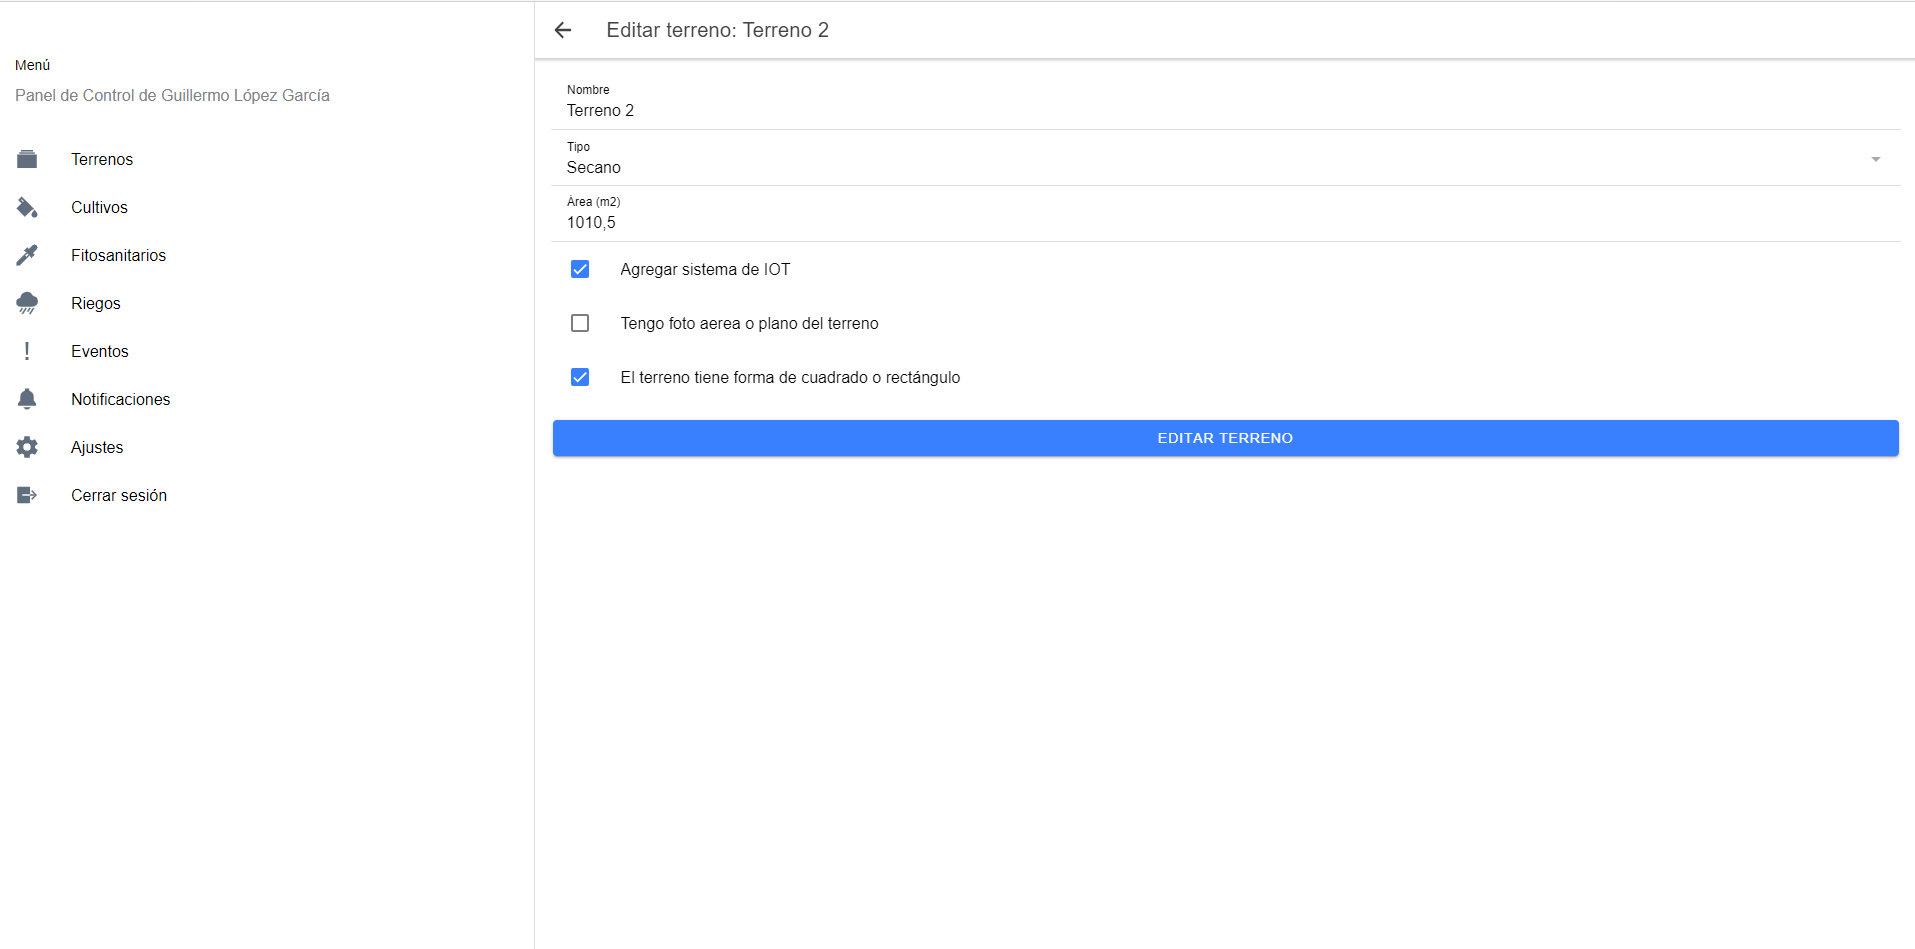
\includegraphics[width=0.7\linewidth]{images/user-manual/farmableland/update.png}
    \caption{Actualizar Terreno}
\end{figure}

\subsubsection{Borrar}
Para borrar un terreno, el usuario debe pulsar en el icono de borrar, el cual aparece resaltado en la Figura 9.9.
Una vez lo pulsé, el terreno se borrará.
\begin{figure}[H]
    \centering
    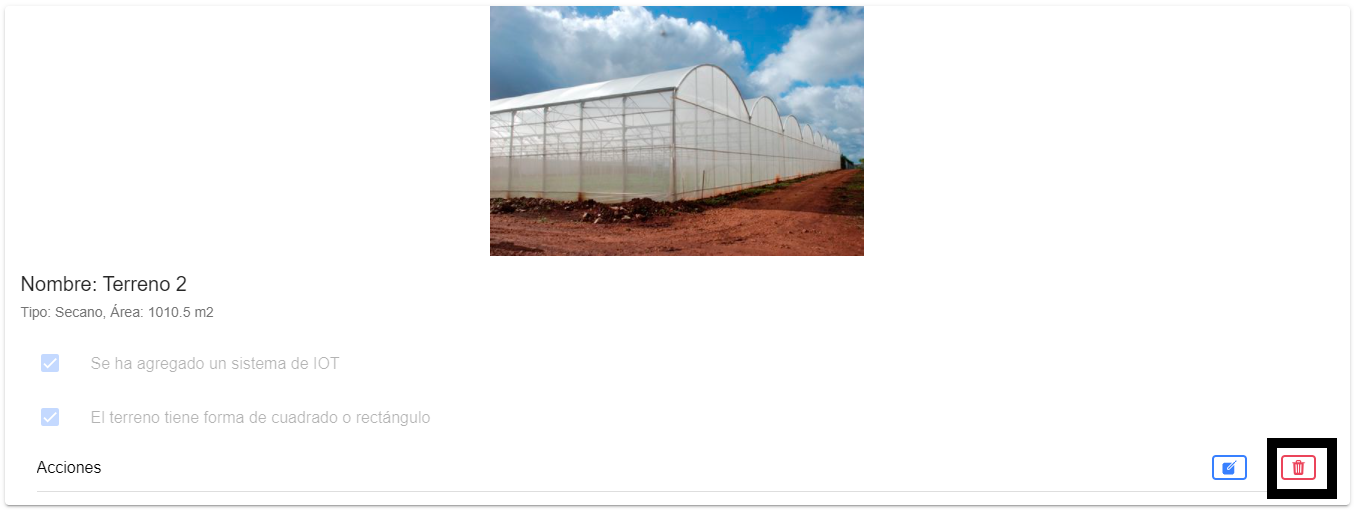
\includegraphics[width=0.7\linewidth]{images/user-manual/farmableland/delete.png}
    \caption{Borrar Terreno}
\end{figure}

\subsection{Cultivos}
En esta sección, se permite todo el CRUD de los cultivos. A continuación, se explica como se hace cada una de las operaciones.

\subsubsection{Listar}
Para listar los cultivos, el usuario debe moverse a la sección de cultivos y directamente se le listará todos los cultivos que posee en sus terrenos, como se puede apreciar en la Figura 9.10.
\begin{figure}[H]
    \centering
    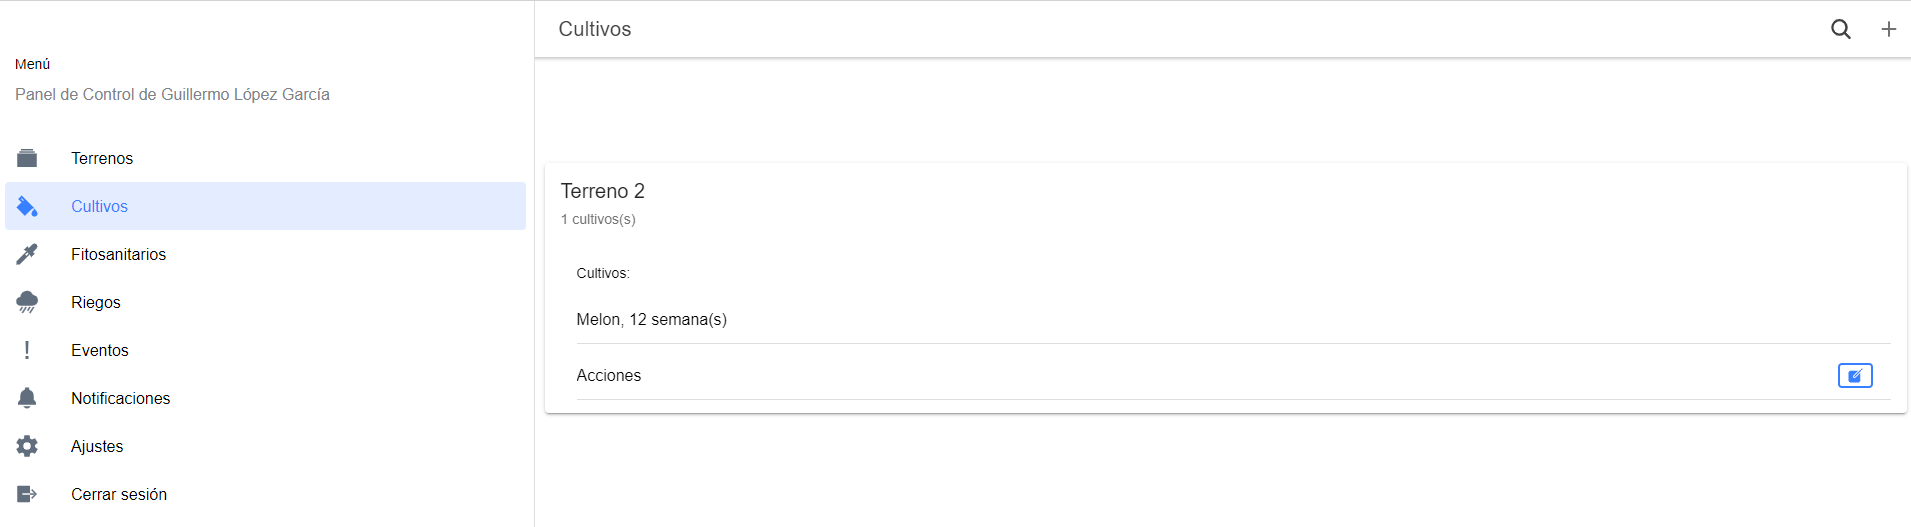
\includegraphics[width=0.7\linewidth]{images/user-manual/crop/list.png}
    \caption{Listar Cultivos}
\end{figure}

\subsubsection{Buscar}
Para buscar un cultivo, el usuario debe pulsar en la barra superior de la sección y escribir la búsqueda deseada. Una vez se escriba la búsqueda, el sistema actualizará el listado de los cultivos automáticamente con el filtro aplicado, como se puede apreciar en la Figura 9.11.
\begin{figure}[H]
    \centering
    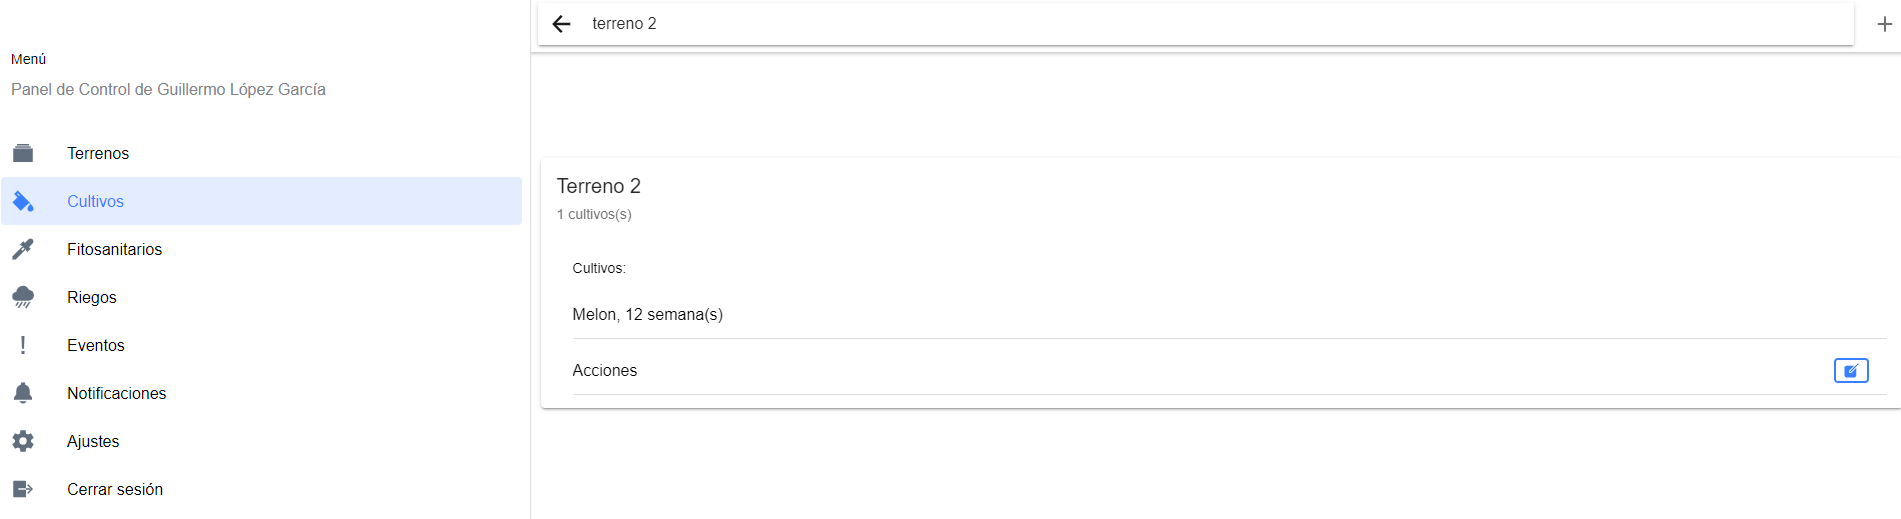
\includegraphics[width=0.7\linewidth]{images/user-manual/crop/search.png}
    \caption{Buscar Cultivos}
\end{figure}

\subsubsection{Añadir}
Para añadir un cultivo, el usuario debe pulsar en el icono con el símbolo ``+'' y el sistema le llevará al formulario correspondiente para crear un cultivo, como se puede apreciar en la Figura 9.12. Una vez complete todos los campos de forma correcta, el sistema guardará el cultivo.
\begin{figure}[H]
    \centering
    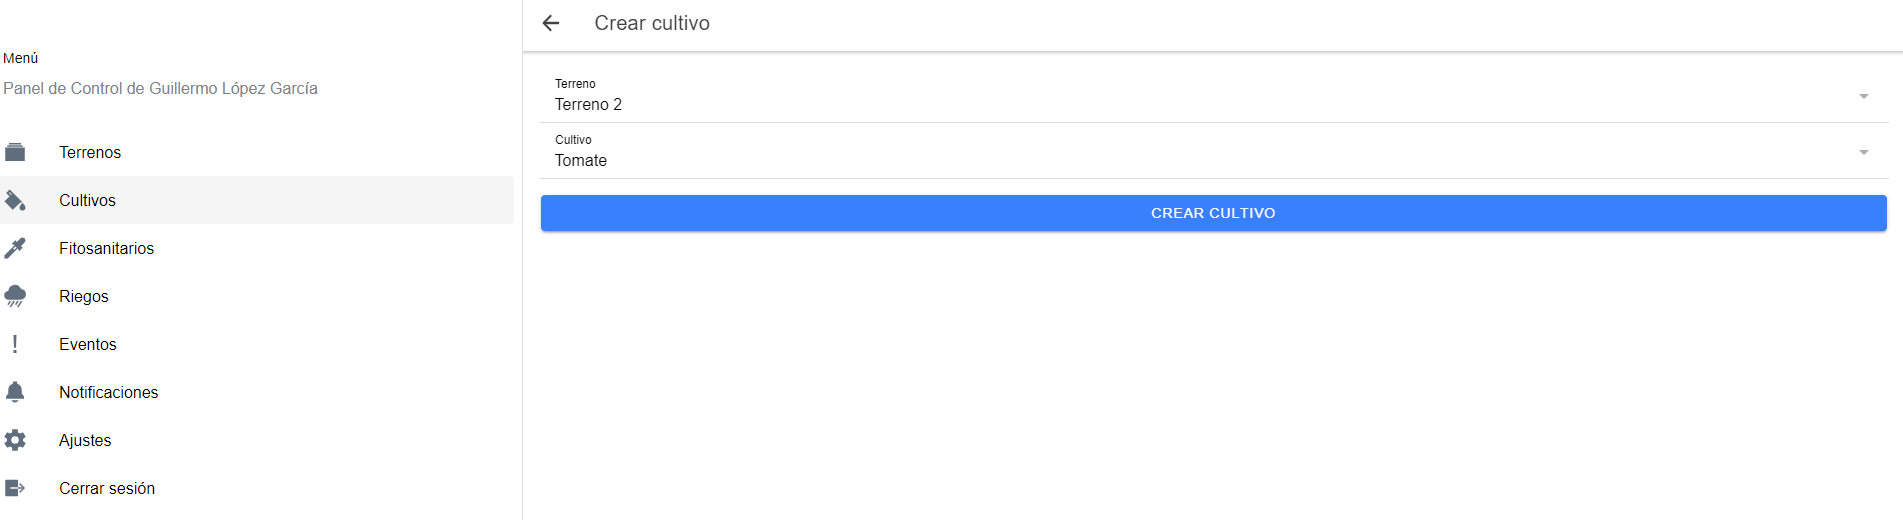
\includegraphics[width=0.7\linewidth]{images/user-manual/crop/create.png}
    \caption{Añadir Cultivo}
\end{figure}

\subsubsection{Modificar}
Para modificar un cultivo, el usuario debe pulsar sobre el icono de editar y el sistema le llevará al formulario correspondiente, que se puede apreciar en la Figura 9.13. Una vez que el usuario edite de forma correcta los campos, el sistema modificará el cultivo.
\begin{figure}[H]
    \centering
    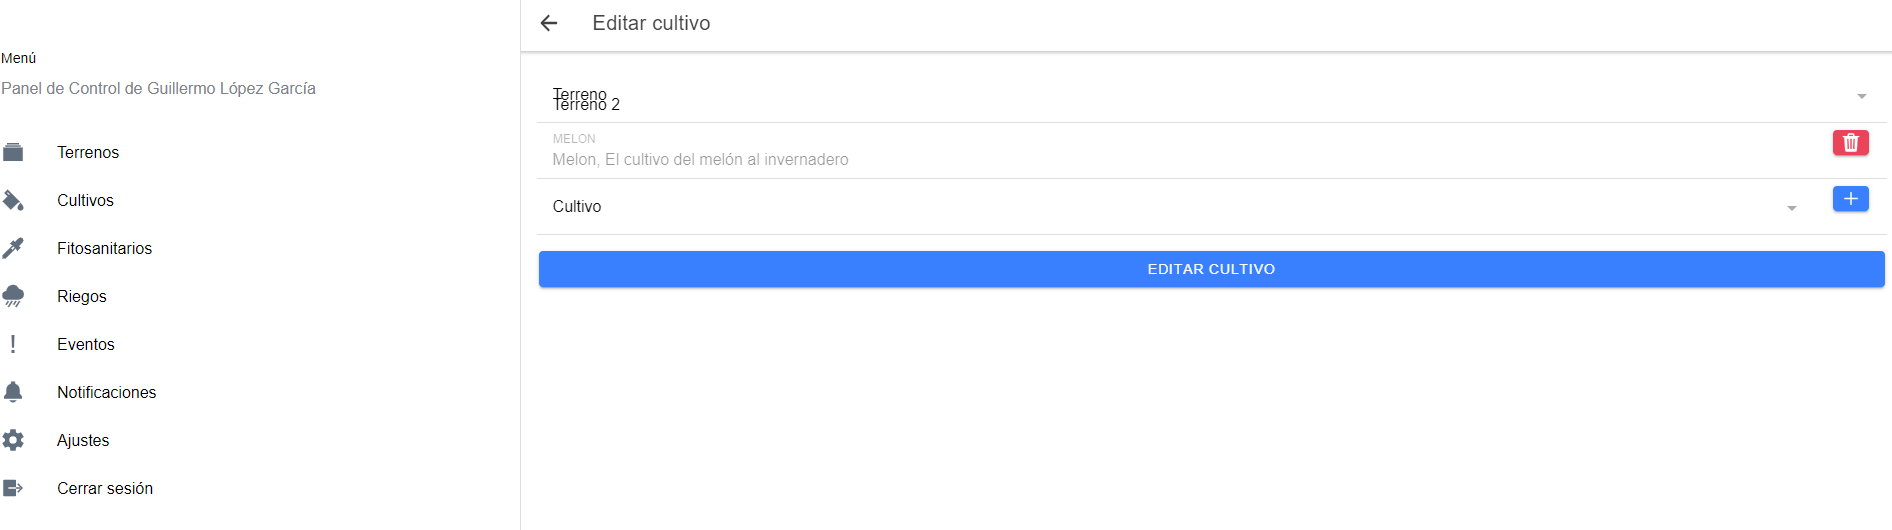
\includegraphics[width=0.7\linewidth]{images/user-manual/crop/update.png}
    \caption{Actualizar Cultivo}
\end{figure}

\subsubsection{Borrar}
Para borrar un cultivo, el usuario debe pulsar sobre el icono de borrar resaltado en la Figura 9.14. Una vez se produzca la acción, el sistema borrará el cultivo del terreno seleccionado.
\begin{figure}[H]
    \centering
    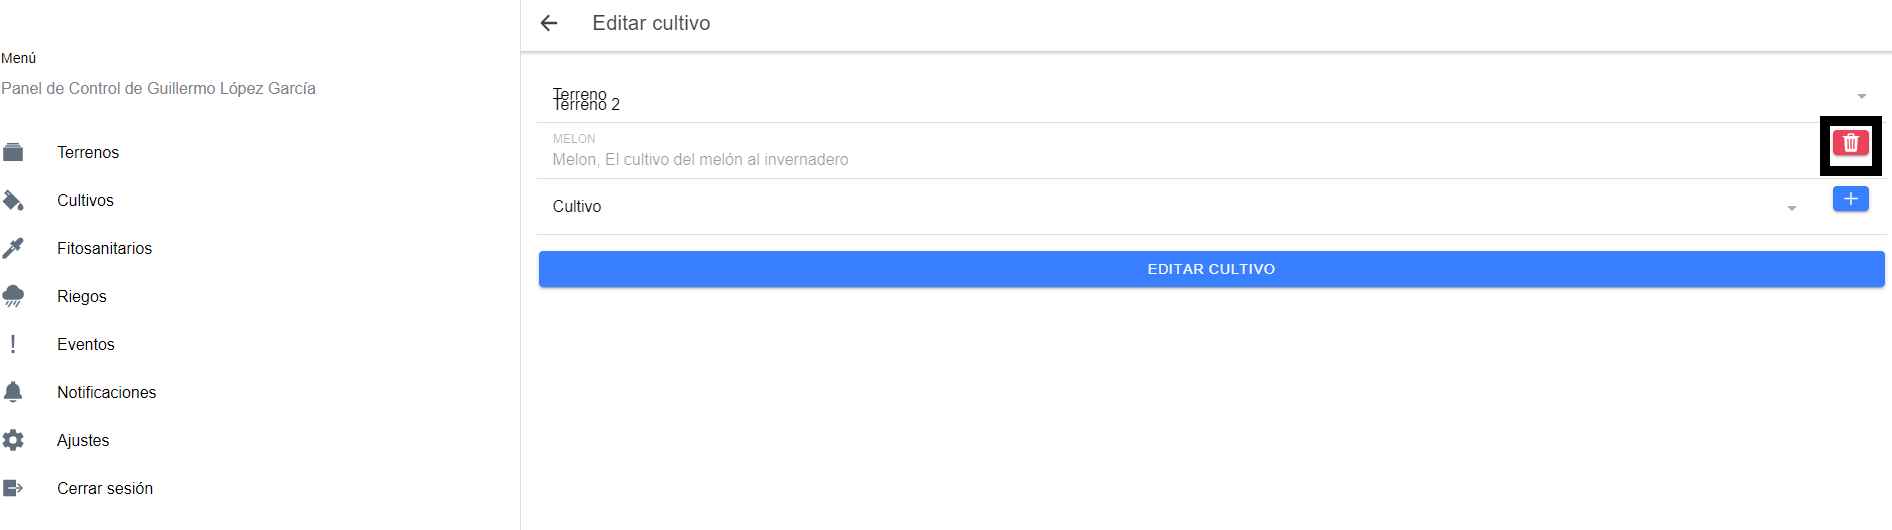
\includegraphics[width=0.7\linewidth]{images/user-manual/crop/delete.png}
    \caption{Borrar Cultivo}
\end{figure}

\subsection{Fitosanitarios}
En esta sección, se permite todo el CRUD de los fitosanitarios. A continuación, se explica como se hace cada una de las operaciones.

\subsubsection{Listar}
Para listar fitosanitarios, el usuario debe moverse a la sección de fitosanitarios pulsando la opción en el menú lateral. Una vez entre, directamente el sistema le listará los fitosanitarios aplicados en cada terreno y en cada cultivo, como se puede apreciar en la Figura 9.15.
\begin{figure}[H]
    \centering
    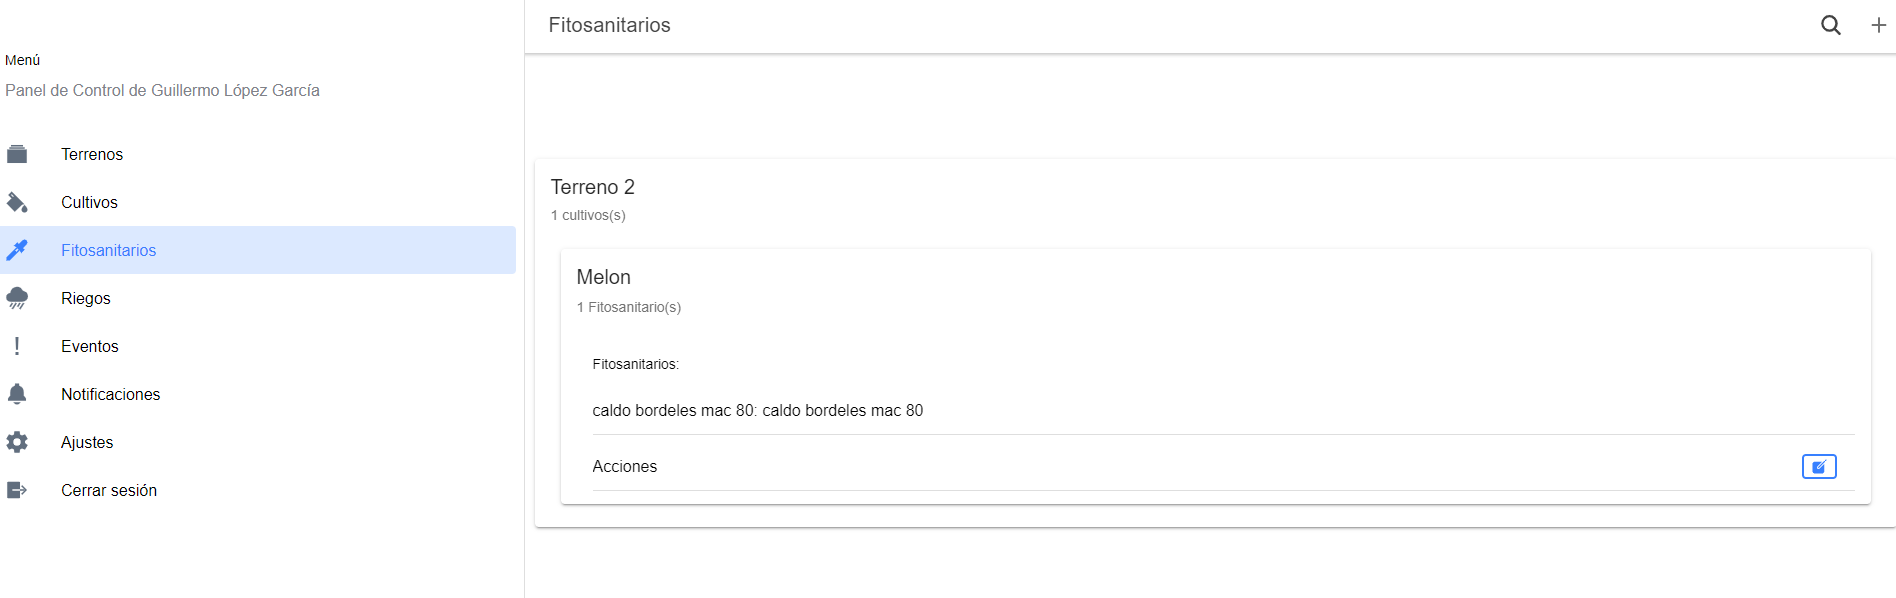
\includegraphics[width=0.7\linewidth]{images/user-manual/phytosanitary/list.png}
    \caption{Listar Fitosanitarios}
\end{figure}

\subsubsection{Buscar}
Para buscar fitosanitarios, el usuario debe pulsar en la barra superior de la sección y escribir el patrón de búsqueda deseado. Una vez lo haga, el sistema automáticamente listará los fitosanitarios con el filtro aplicado, como se puede apreciar en la Figura 9.16.
\begin{figure}[H]
    \centering
    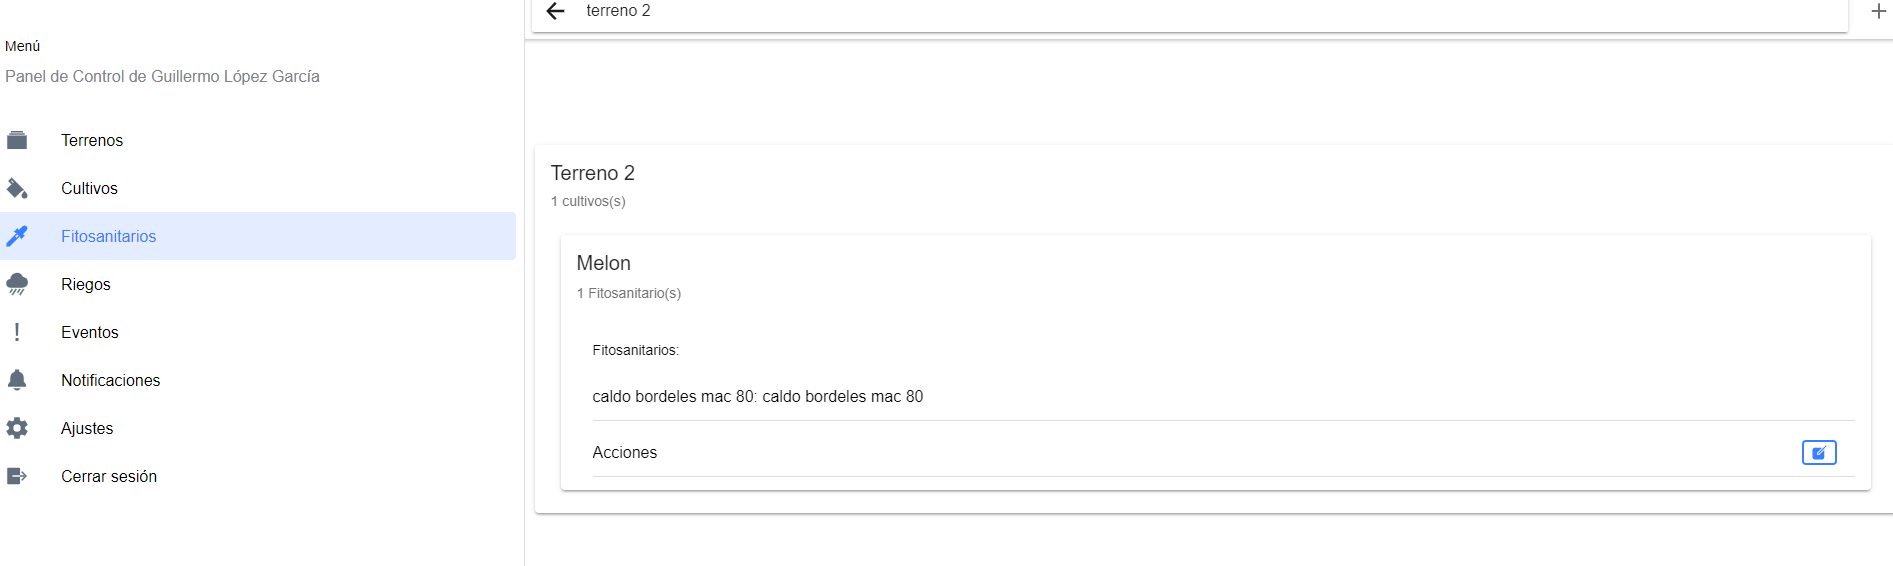
\includegraphics[width=0.7\linewidth]{images/user-manual/phytosanitary/search.png}
    \caption{Buscar Fitosanitarios}
\end{figure}

\subsubsection{Añadir}
Para añadir un fitosanitario, el usuario debe pulsar sobre el icono con el símbolo ``+''. Una vez lo haga, el sistema lo llevará para el formulario correspondiente, que se puede apreciar en la Figura 9.17. Una vez complete todos los campos de forma correcta, se añadirá el fitosanitario.
\begin{figure}[H]
    \centering
    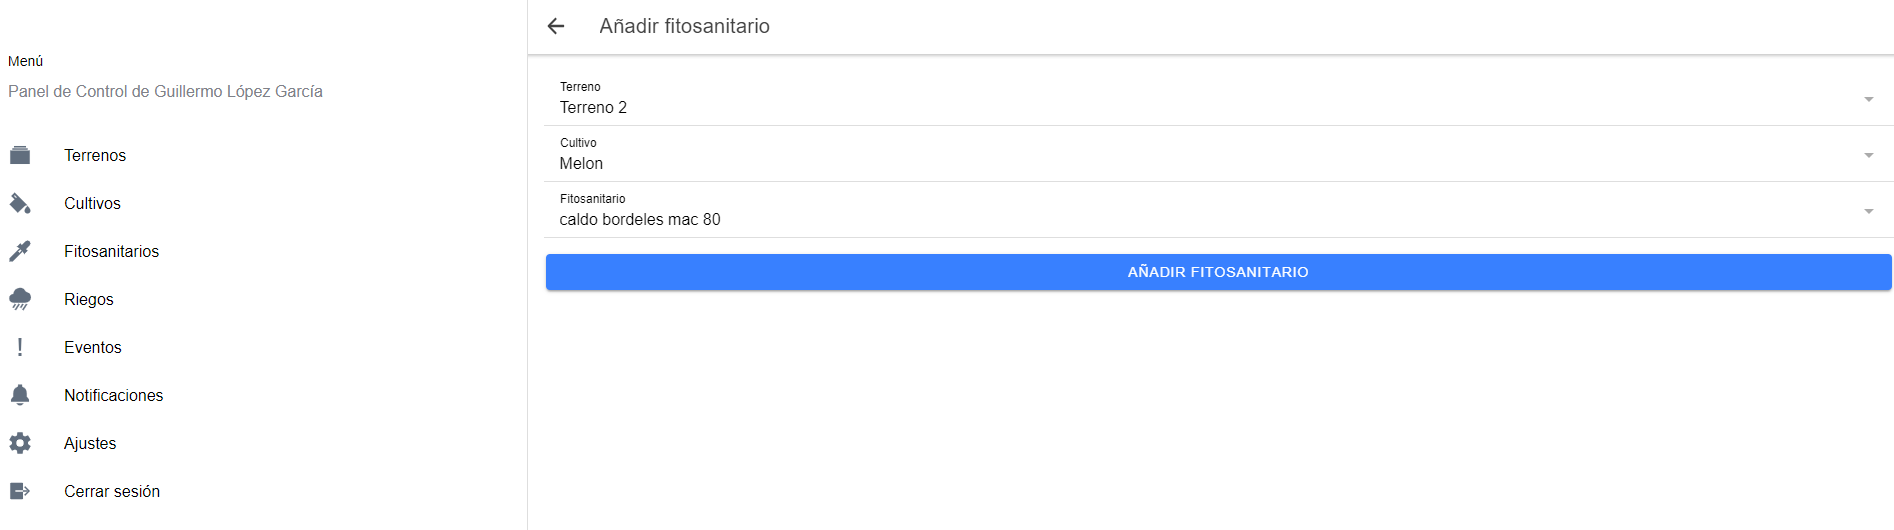
\includegraphics[width=0.7\linewidth]{images/user-manual/phytosanitary/create.png}
    \caption{Añadir Fitosanitario}
\end{figure}

\subsubsection{Modificar}
Para modificar un fitosanitario, el usuario debe pulsar sobre el icono de editar. Una vez lo haga, el sistema lo enviará al formulario correspondiente, que se puede apreciar en la Figura 9.18. Cuando el usuario modifique los campos que desee de forma correcta, el sistema guardará al fitosanitario.
\begin{figure}[H]
    \centering
    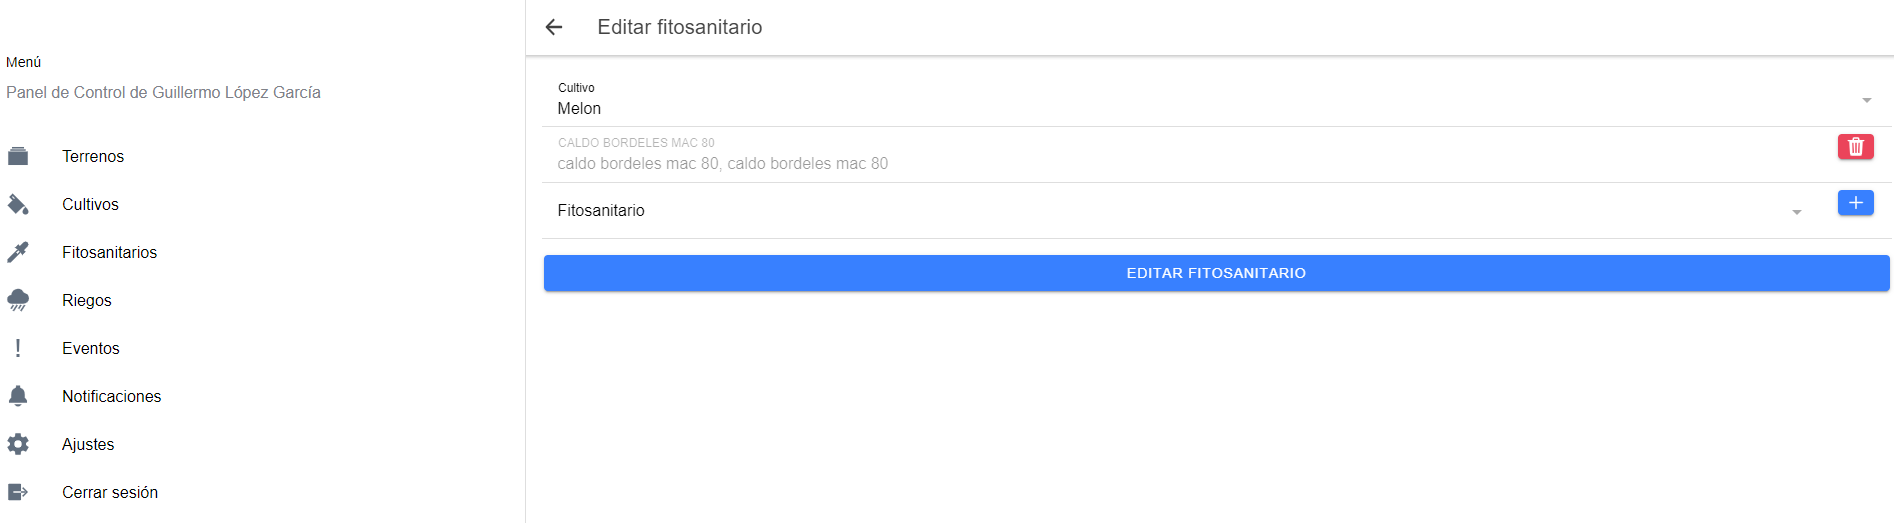
\includegraphics[width=0.7\linewidth]{images/user-manual/phytosanitary/update.png}
    \caption{Actualizar Fitosanitario}
\end{figure}

\subsubsection{Borrar}
Para borrar un fitosanitario, el usuario debe pulsar sobre el icono de borrar, el cual está resaltado en la Figura 9.19. Una vez el usuario pulse sobre el icono, el fitosanitario se borrará.
\begin{figure}[H]
    \centering
    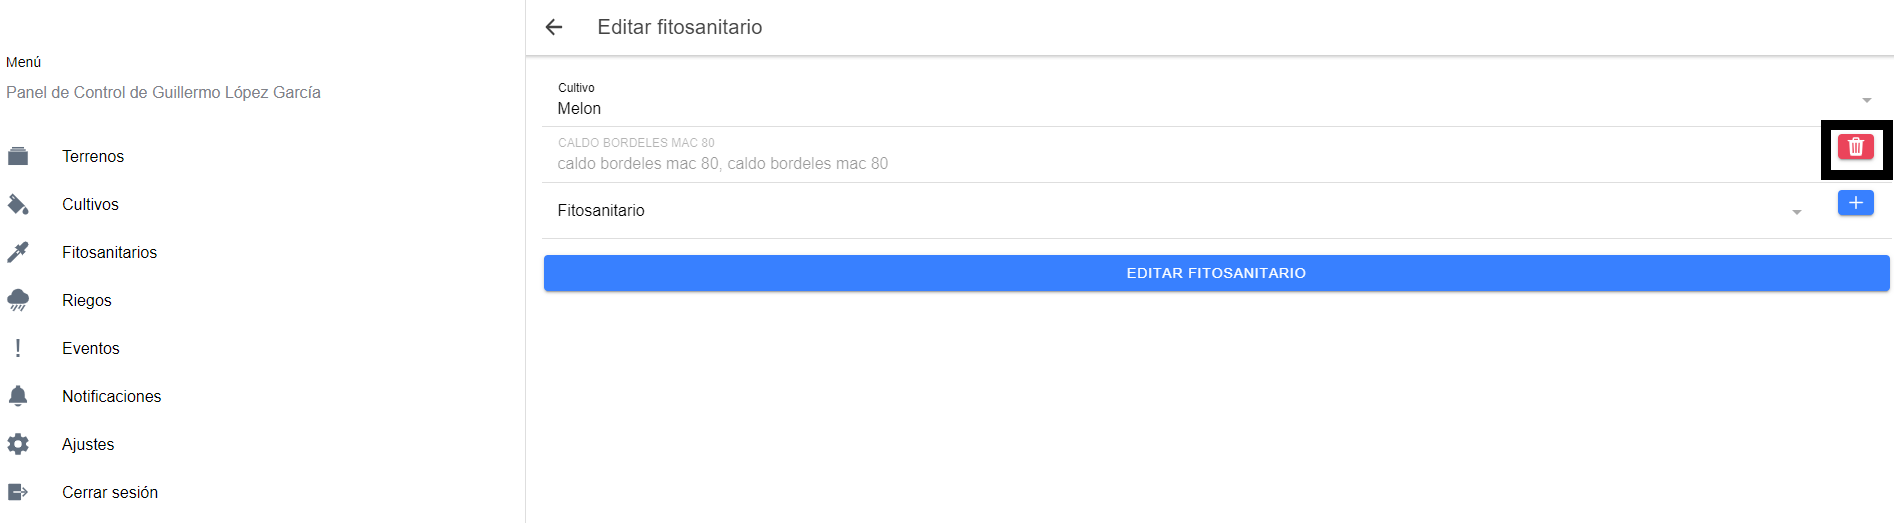
\includegraphics[width=0.7\linewidth]{images/user-manual/phytosanitary/delete.png}
    \caption{Borrar Fitosanitario}
\end{figure}

\subsection{Riegos}
En esta sección, se permite todo el CRUD de los riegos. A continuación, se explica como se hace cada una de las operaciones.

\subsubsection{Listar}
Para listar los riegos, el usuario debe moverse a la sección mediante el menú lateral. Una vez entre en dicha sección, el sistema automáticamente mostrará todos los riegos del usuario, como se puede apreciar en la Figura 9.20.
\begin{figure}[H]
    \centering
    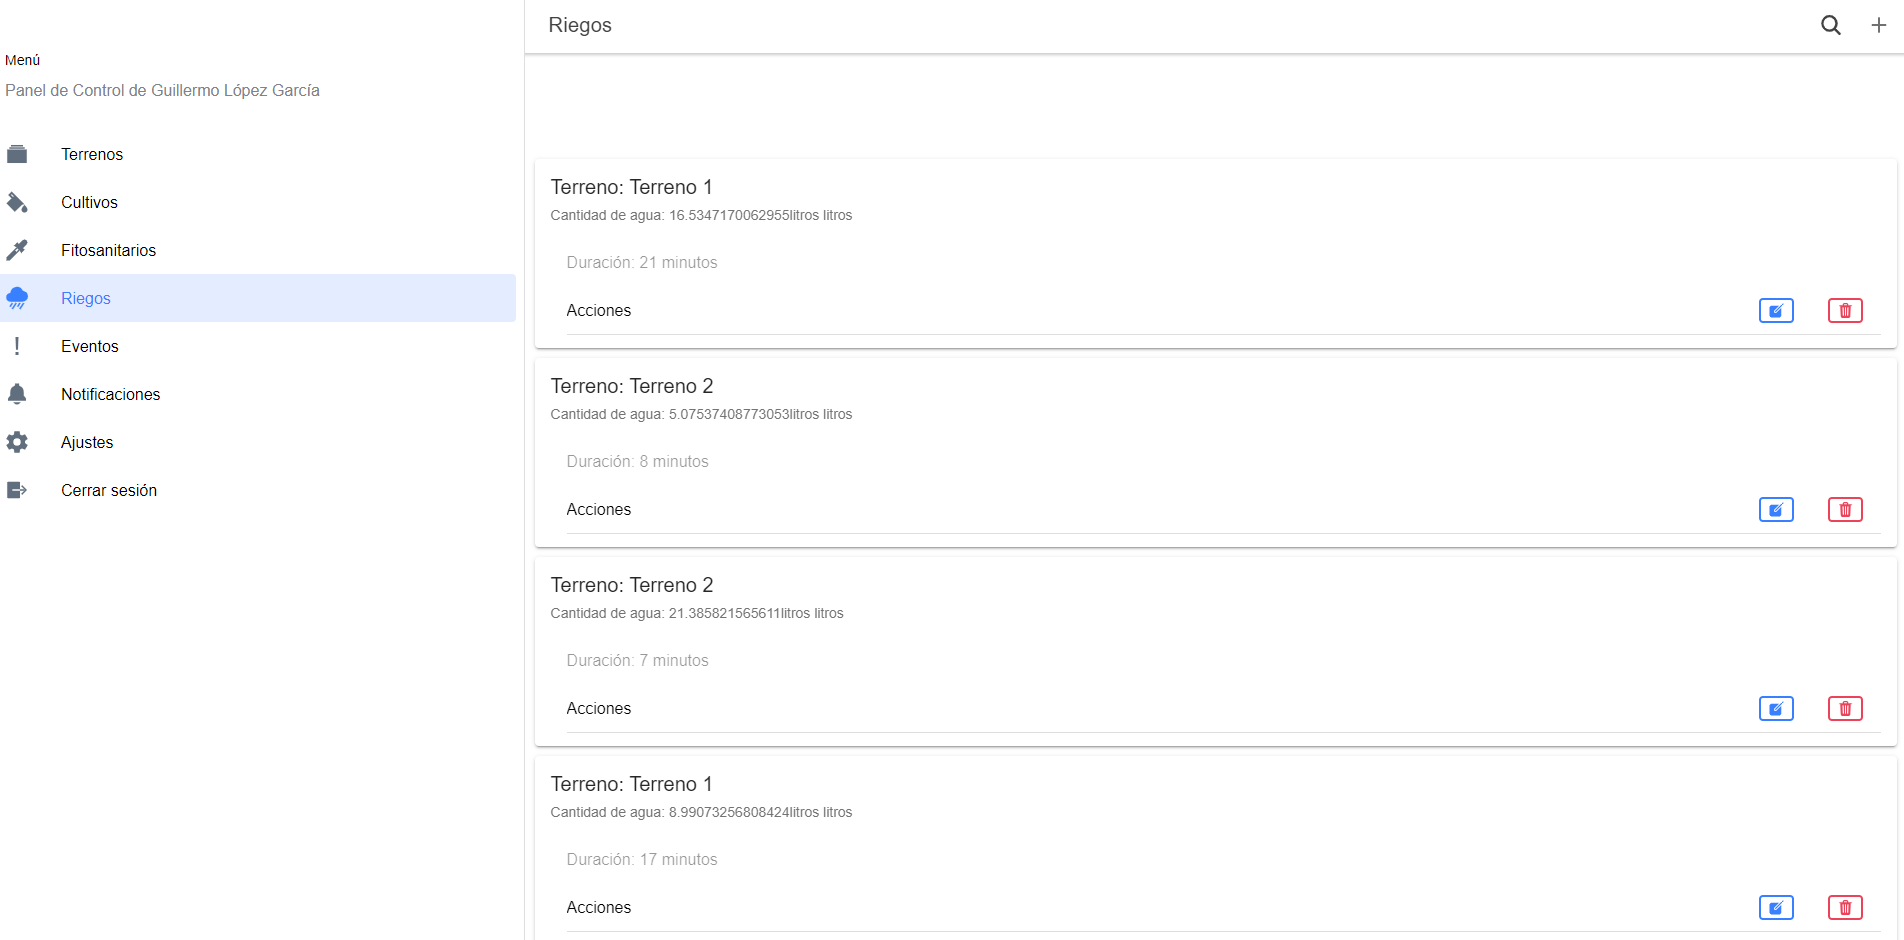
\includegraphics[width=0.7\linewidth]{images/user-manual/irrigate/list.png}
    \caption{Listar Riegos}
\end{figure}

\subsubsection{Buscar}
Para buscar riegos, el usuario debe pulsar sobre la barra superior de la sección y escribir la búsqueda deseada. El sistema, automáticamente, volverá a listar los riegos con el filtro aplicado, como se puede apreciar en la Figura 9.21.
\begin{figure}[H]
    \centering
    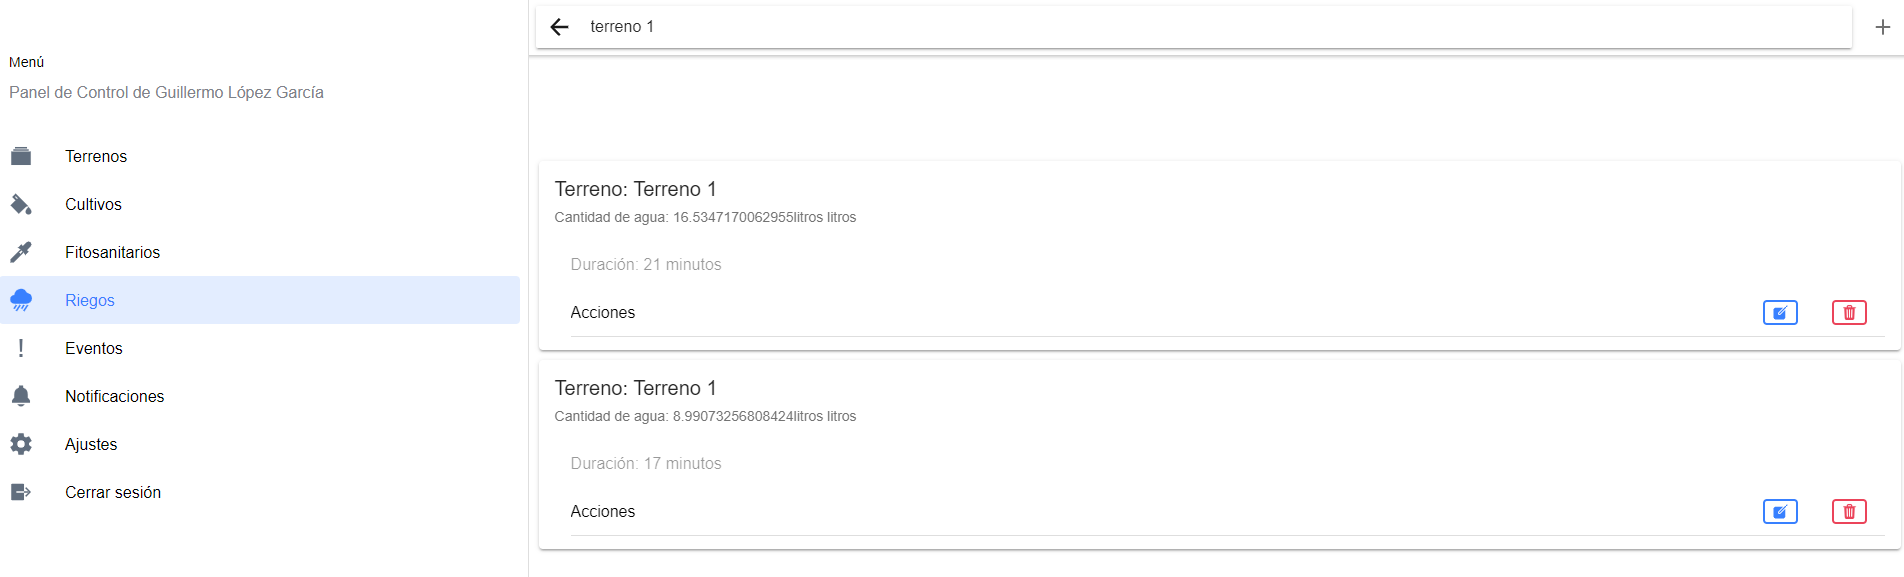
\includegraphics[width=0.7\linewidth]{images/user-manual/irrigate/search.png}
    \caption{Buscar Riegos}
\end{figure}

\subsubsection{Añadir}
Para añadir un riego, el usuario debe pulsar sobre el icono con el símbolo ``+'' y el sistema lo llevará al formulario correspondiente, que se puede apreciar en la Figura 9.22. Una vez el usuario rellene los campos de forma correcta, el sistema guardará el riego.
\begin{figure}[H]
    \centering
    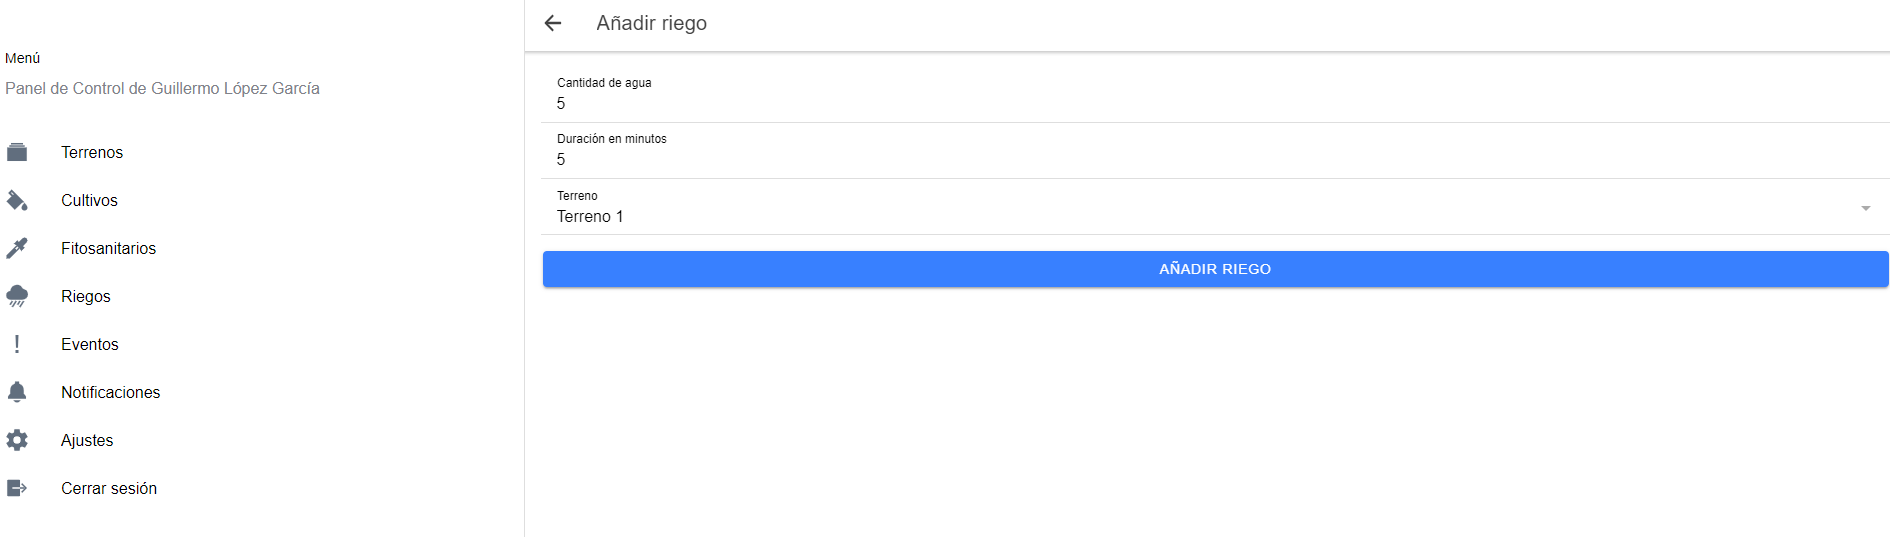
\includegraphics[width=0.7\linewidth]{images/user-manual/irrigate/create.png}
    \caption{Añadir Riego}
\end{figure}

\subsubsection{Modificar}
Para modificar un riego, el usuario debe pulsar sobre el icono de editar, y el sistema llevará al usuario al formulario correspondiente, que se puede apreciar en la Figura 9.23. Una vez el usuario modifique los campos, el sistema guadará el riego modificado.
\begin{figure}[H]
    \centering
    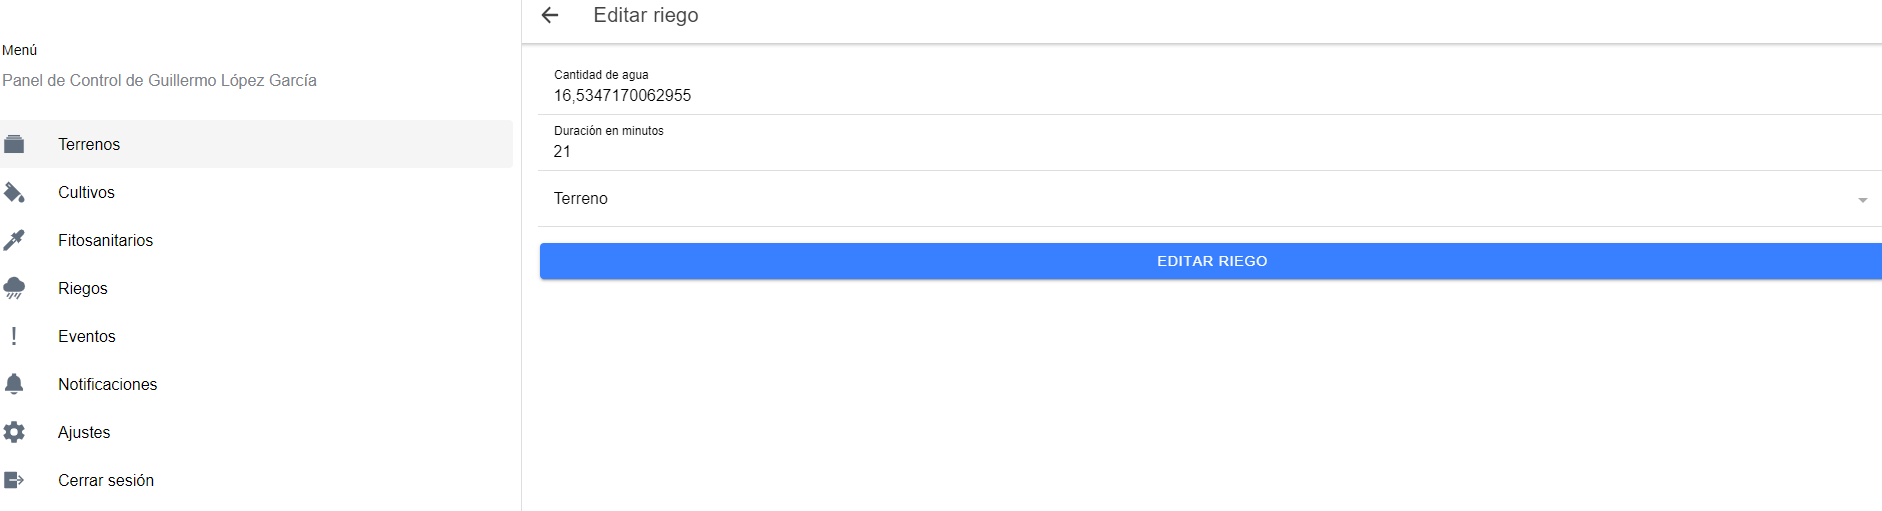
\includegraphics[width=0.7\linewidth]{images/user-manual/irrigate/update.png}
    \caption{Actualizar Riego}
\end{figure}

\subsubsection{Borrar}
Para borrar un riego, el usuario debe pulsar sobre el icono de borrar, resaltado en la Figura 9.24. Una vez pulse en el, el sistema borrará el riego.
\begin{figure}[H]
    \centering
    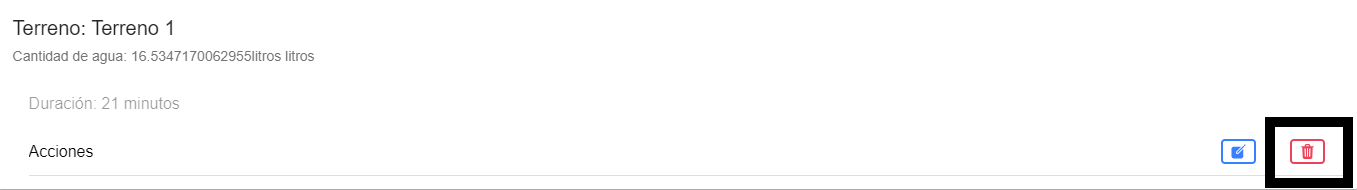
\includegraphics[width=0.7\linewidth]{images/user-manual/irrigate/delete.png}
    \caption{Borrar Riego}
\end{figure}

\subsection{Eventos}
En esta sección, se permite todo el CRUD de los eventos. A continuación, se explica como se hace cada una de las operaciones.

\subsubsection{Listar}
Para listar los eventos a los que está suscrito, el usuario deberá moverse a la sección de eventos. Una vez entre en la sección, el sistema automáticamente listará todos los eventos complejos a los que está suscrito el usuario. Esto se puede apreciar en la Figura 9.25.
\begin{figure}[H]
    \centering
    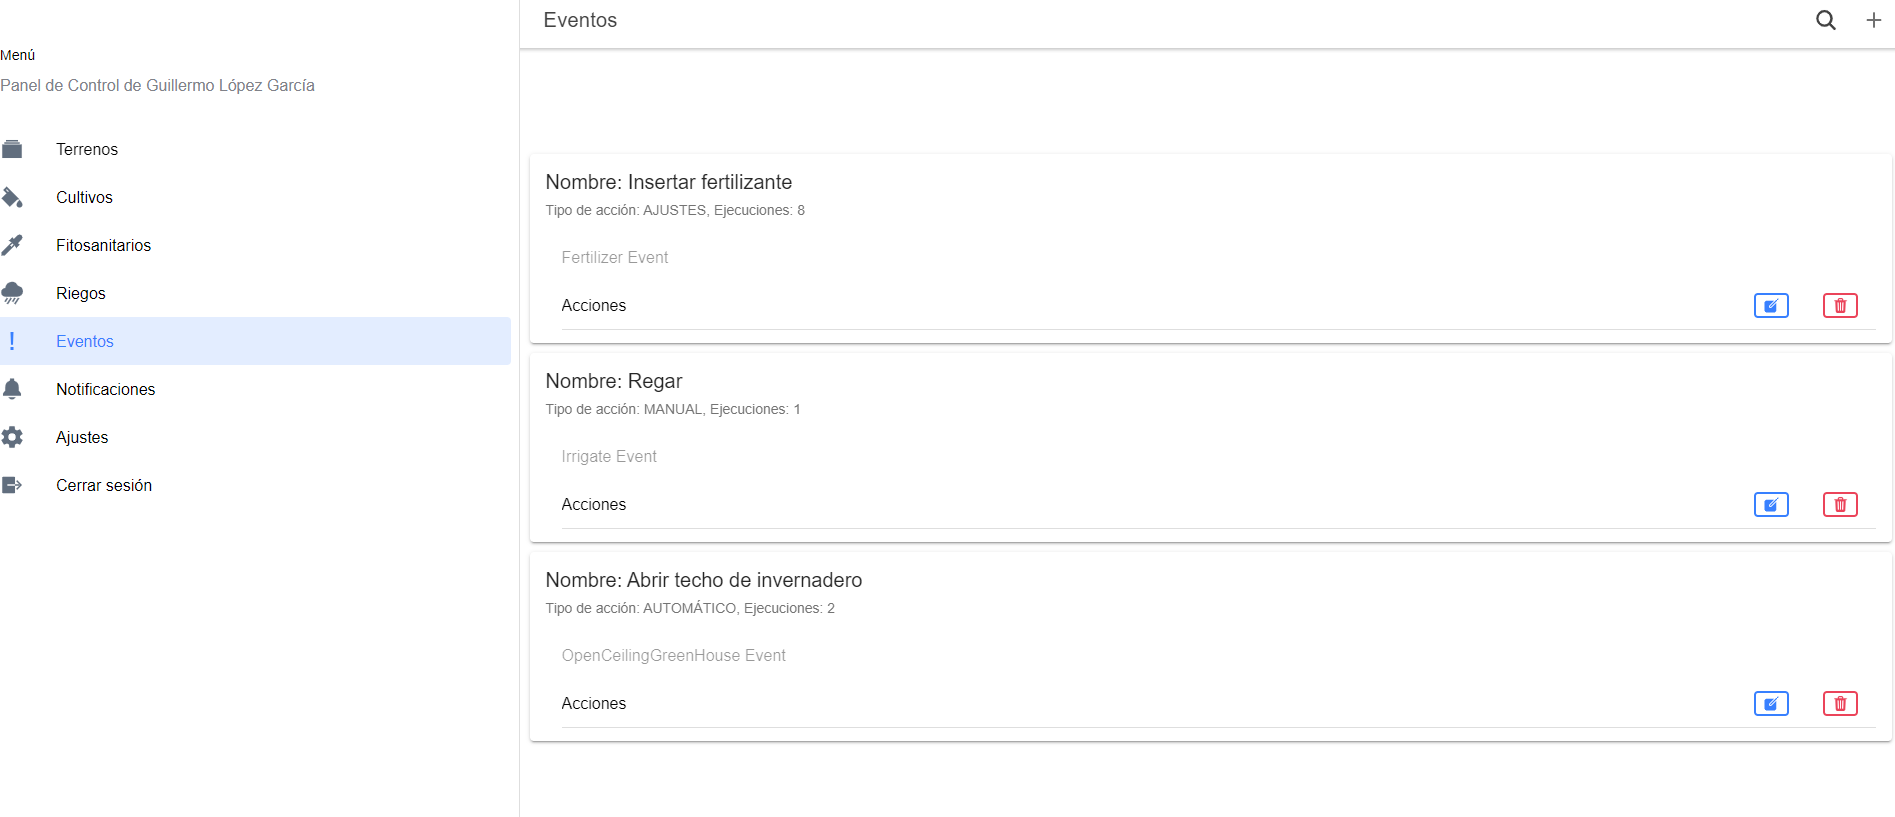
\includegraphics[width=0.7\linewidth]{images/user-manual/events/list.png}
    \caption{Listar Eventos}
\end{figure}

\subsubsection{Buscar}
Para buscar entre los eventos complejos, el usuario debe pulsar sobre la barra superior de la sección. una vez lo haga, deberá escribir la búsqueda que desea. El sistema automáticamente, listará los eventos con el filtro aplicado, como se puede apreciar en la Figura 9.26.
\begin{figure}[H]
    \centering
    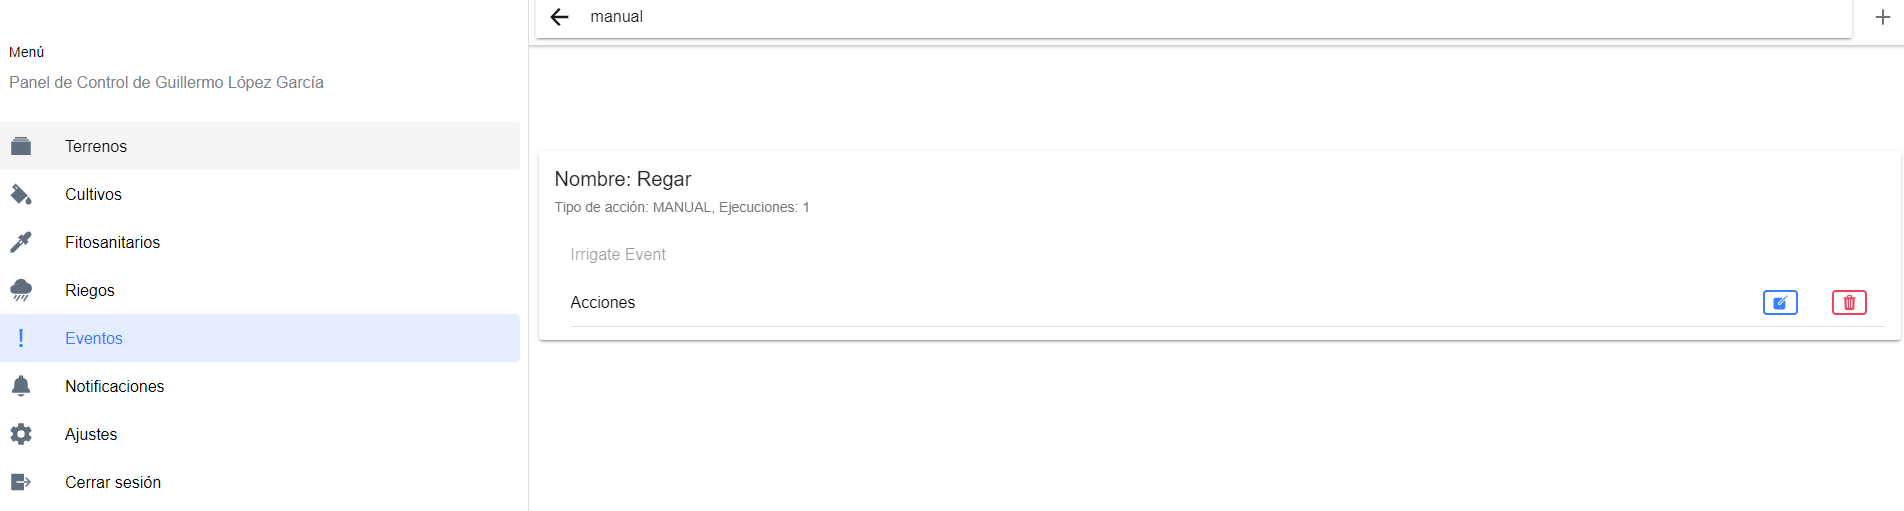
\includegraphics[width=0.7\linewidth]{images/user-manual/events/search.png}
    \caption{Buscar Eventos}
\end{figure}

\subsubsection{Añadir}
Para suscribirse a un evento complejo, el usuario deberá pulsar sobre el icono con el símbolo ``+'' y el sistema le llevará al formulario correspondiente como se puede apreciar en la Figura 9.27. Una vez el usuario rellene el formulario correctamente, el sistema guardará la suscripción al evento.
\begin{figure}[H]
    \centering
    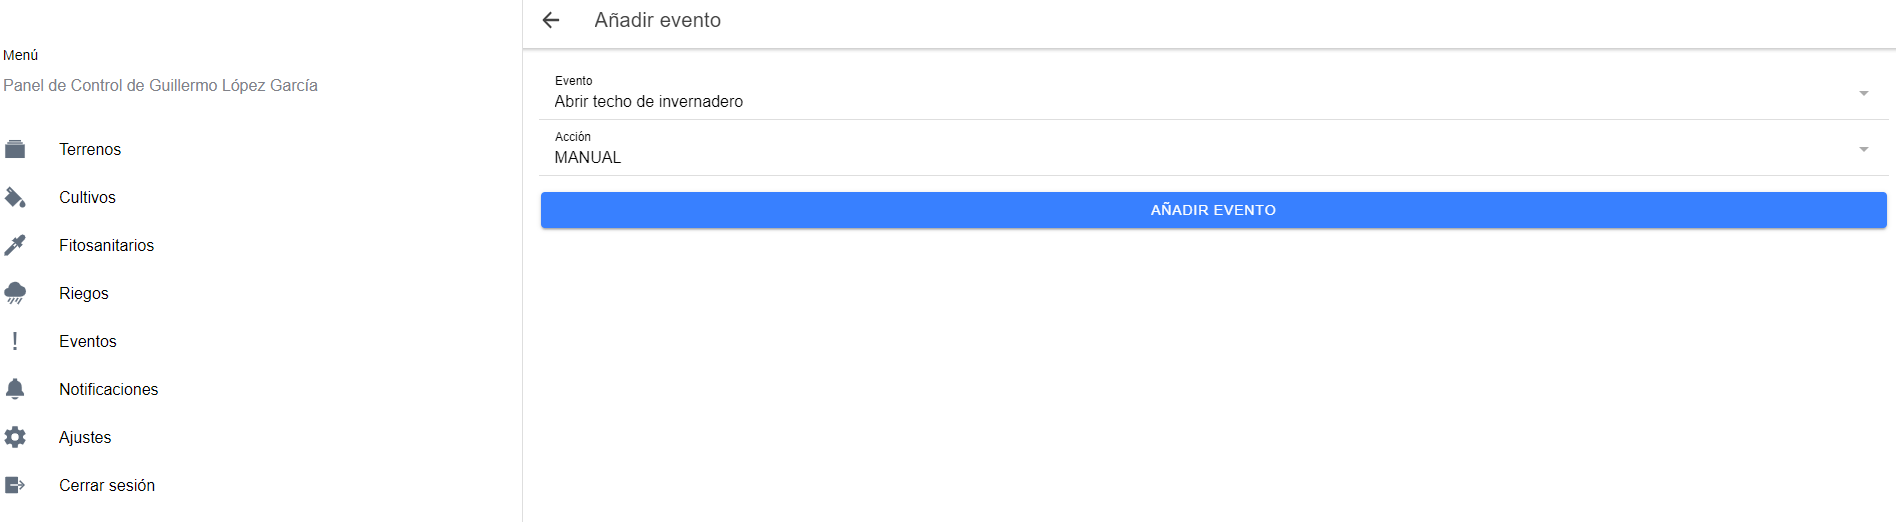
\includegraphics[width=0.7\linewidth]{images/user-manual/events/create.png}
    \caption{Añadir Evento}
\end{figure}

\subsubsection{Modificar}
Para modificar la suscripción a un evento, el usuario deberá pulsar sobre el icono de editar. Una vez pulse, el sistema llevará al usuario al formulario correspondiente que se puede apreciar en la Figura 9.28. Cuando el usuario modifique los campos, el sistema guardará la suscripción modificada.
\begin{figure}[H]
    \centering
    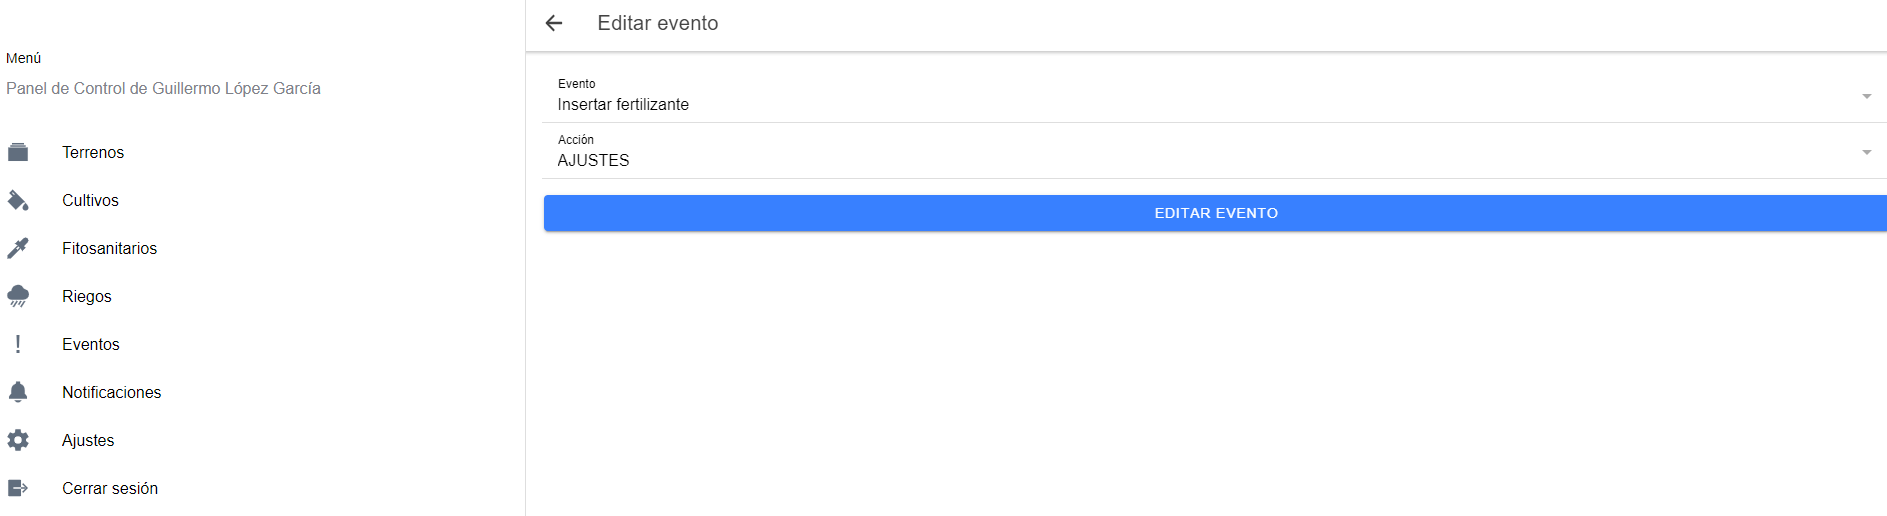
\includegraphics[width=0.7\linewidth]{images/user-manual/events/update.png}
    \caption{Actualizar Evento}
\end{figure}

\subsubsection{Borrar}
Para desuscribirse de un evento complejo, el usuario deberá pulsar sobre el icono de borrar que está resaltado en la Figura 9.29. Una vez el usuario pulse, se borrará la suscripción del usuario a dicho evento complejo.
\begin{figure}[H]
    \centering
    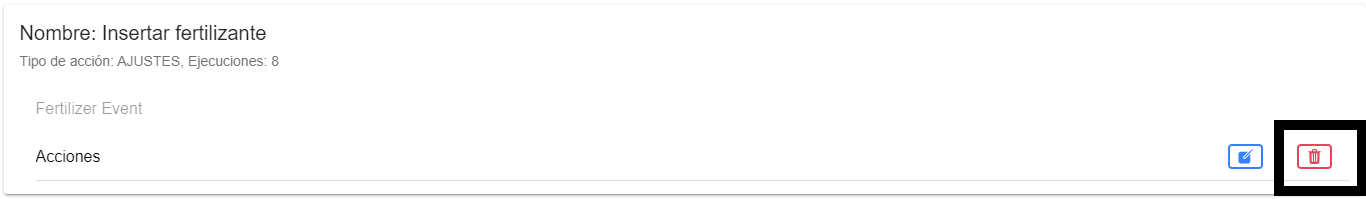
\includegraphics[width=0.7\linewidth]{images/user-manual/events/delete.png}
    \caption{Borrar Evento}
\end{figure}

\subsection{Notificaciones}
En esta sección, se permite listar todo el histórico de notificaciones del usuario.

\subsubsection{Listar}
Para listar las notificaciones, el usuario deberá moverse a la sección. Una vez se encuentre en ella, el sistema automáticamente mostrará todas las notificaciones del usuario ordenadas de más cercana a más lejana en el tiempo, como se puede apreciar en la Figura 9.30.
\begin{figure}[H]
    \centering
    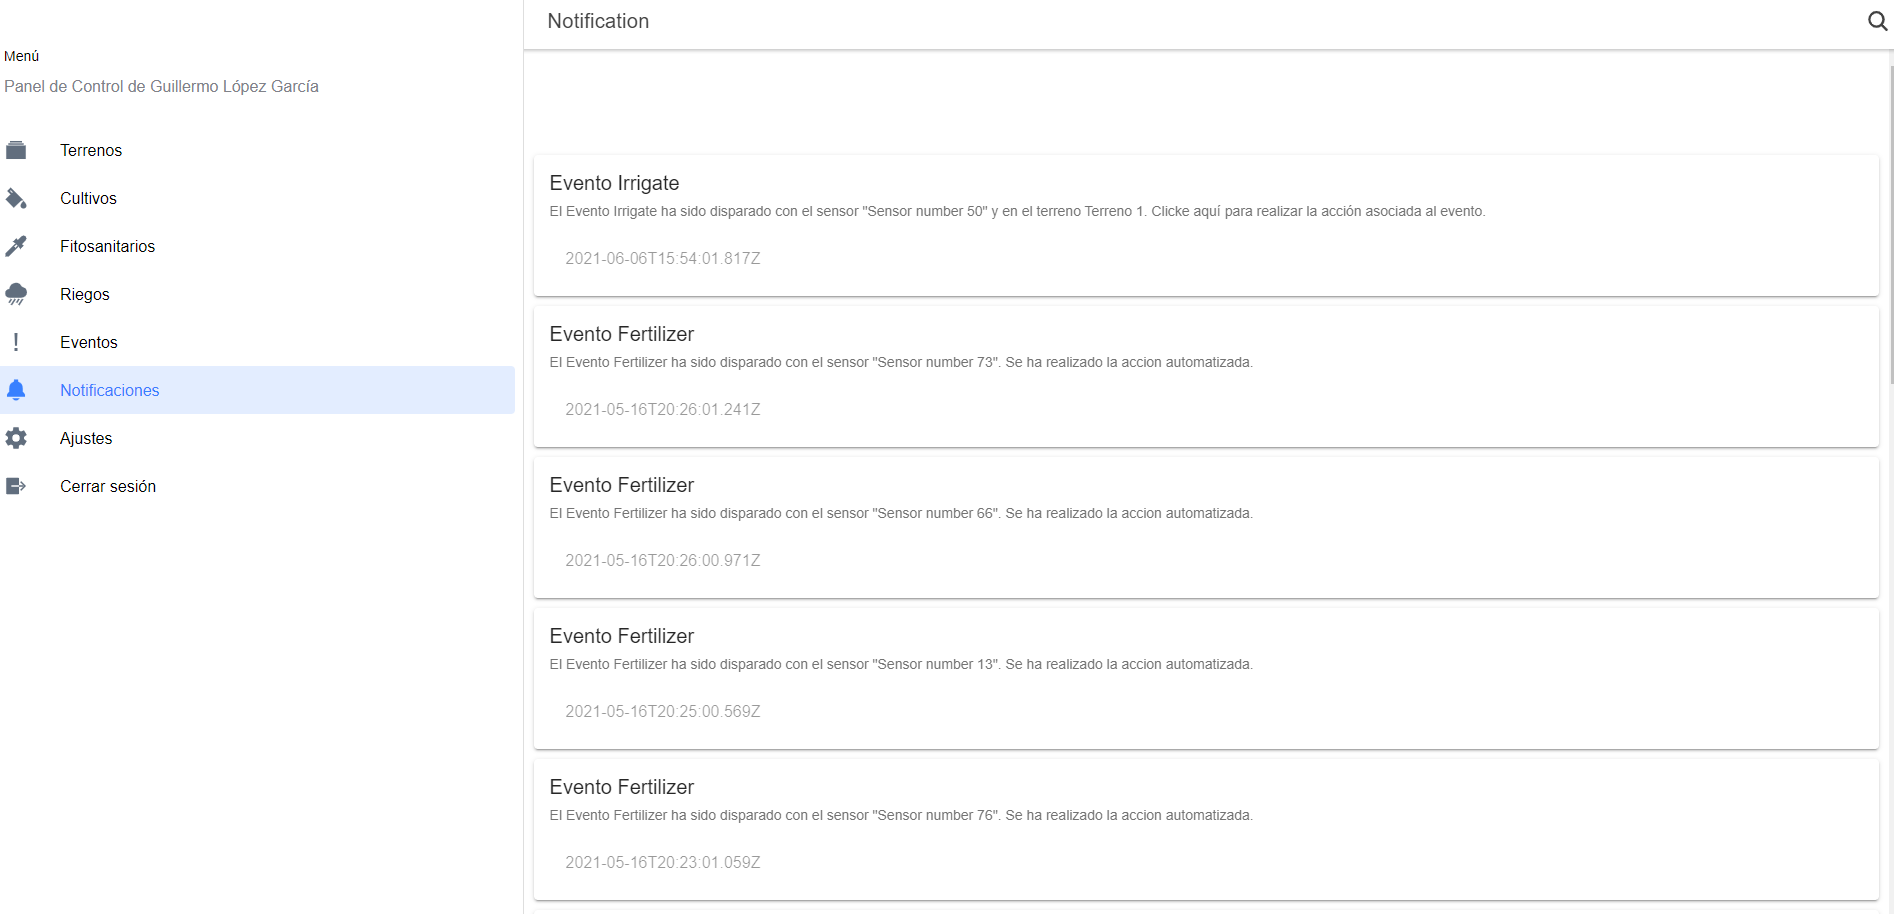
\includegraphics[width=0.7\linewidth]{images/user-manual/notifications/list.png}
    \caption{Listar Notificaciones}
\end{figure}

\subsubsection{Buscar}
Para buscar notificaciones, el usuario deberá pulsar en la barra superior de la sección. Una vez lo haga, el usuario deberá escribir su búsqueda. El sistema automáticamente volverá a listar las notificaciones con el filtro aplicado, como se puede apreciar en la Figura 9.31.
\begin{figure}[H]
    \centering
    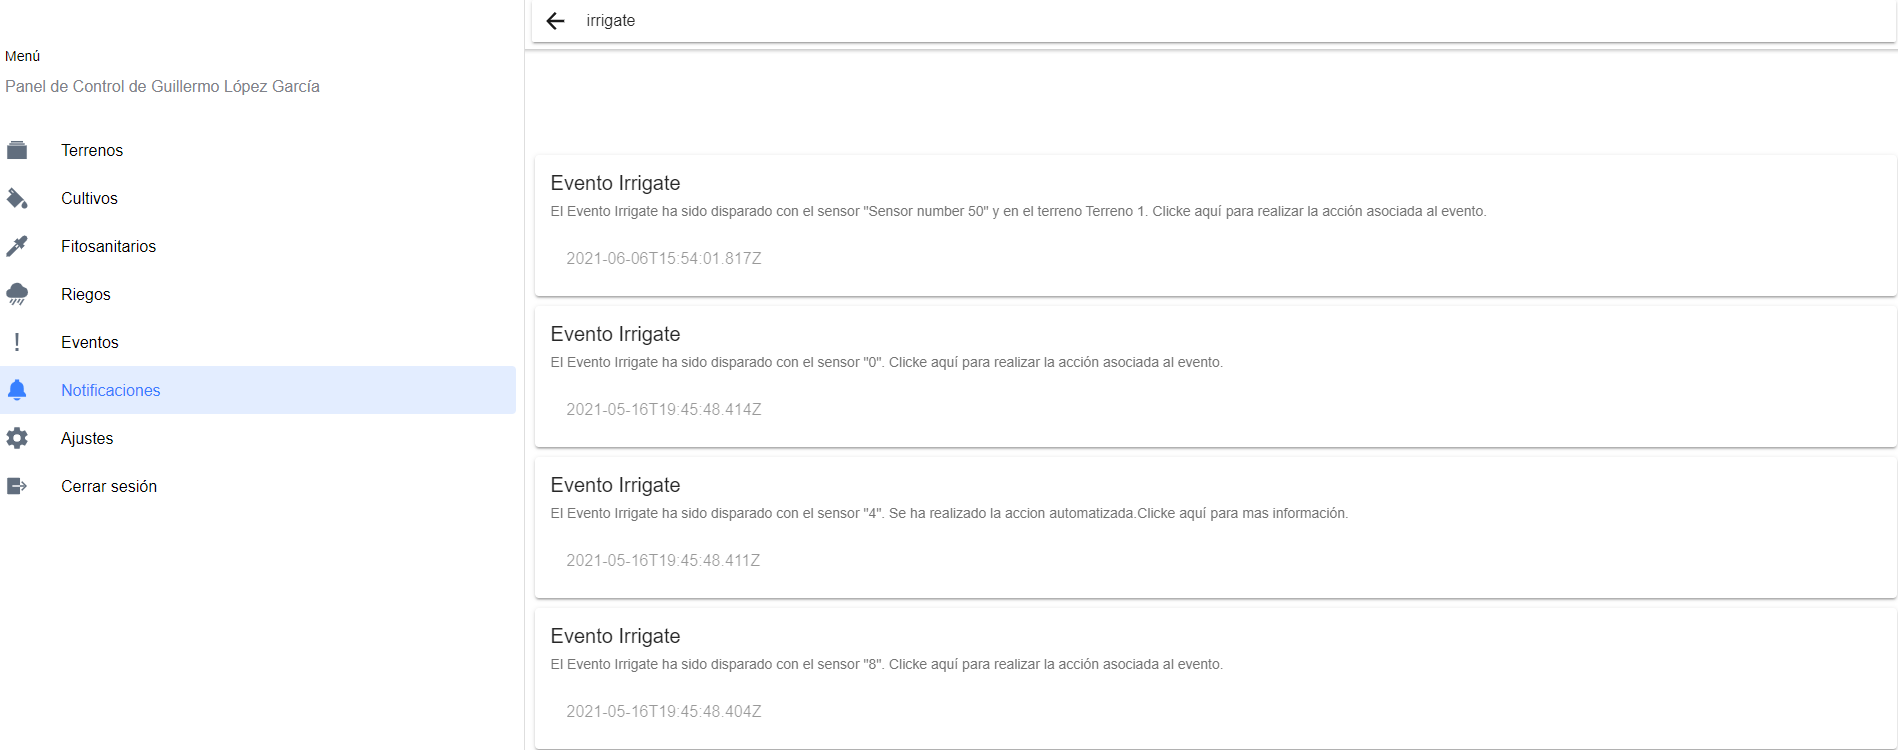
\includegraphics[width=0.7\linewidth]{images/user-manual/notifications/search.png}
    \caption{Buscar Notificaciones}
\end{figure}

\subsection{Ajustes}
En esta sección, se permite ver y modificar todos los ajustes del sistema de los usuarios.

\subsubsection{Ver}
Para ver los ajustes, el usuario deberá moverse a la sección usando el menú lateral. Una vez este en la sección, el sistema mostrará al usuario todas sus opciones de ajustes y los valores actuales. Esto se puede apreciar en la Figura 9.32.
\begin{figure}[H]
    \centering
    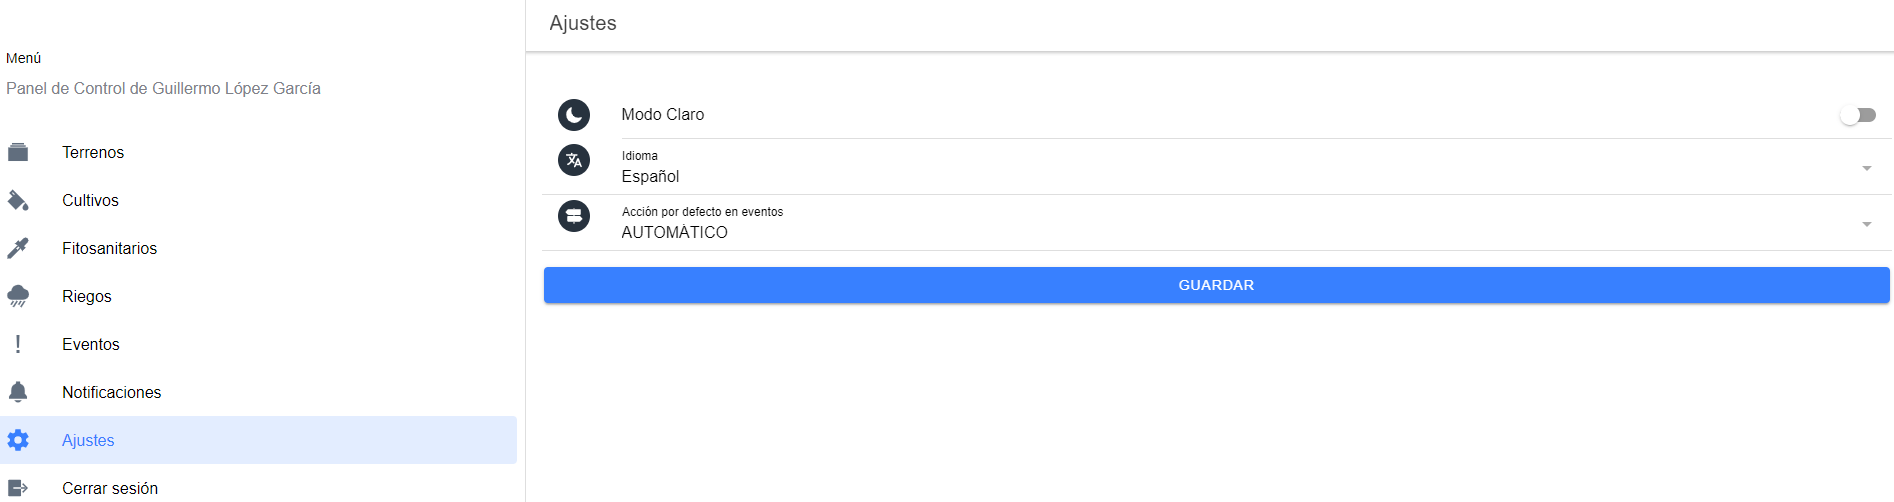
\includegraphics[width=0.7\linewidth]{images/user-manual/settings/list.png}
    \caption{Ver Ajustes}
\end{figure}

\subsubsection{Modificar}
Para modificar los ajustes del sistema, el usuario deberá entrar en la sección de ajustes y modificar los valores en los diferentes campos existentes. Una vez lo haya modificado, al pulsar sobre el botón ``Guardar'', el sistema guardará los nuevos valores de los ajustes del sistema del usuario, como se aprecia en la Figura 9.33.
\begin{figure}[H]
    \centering
    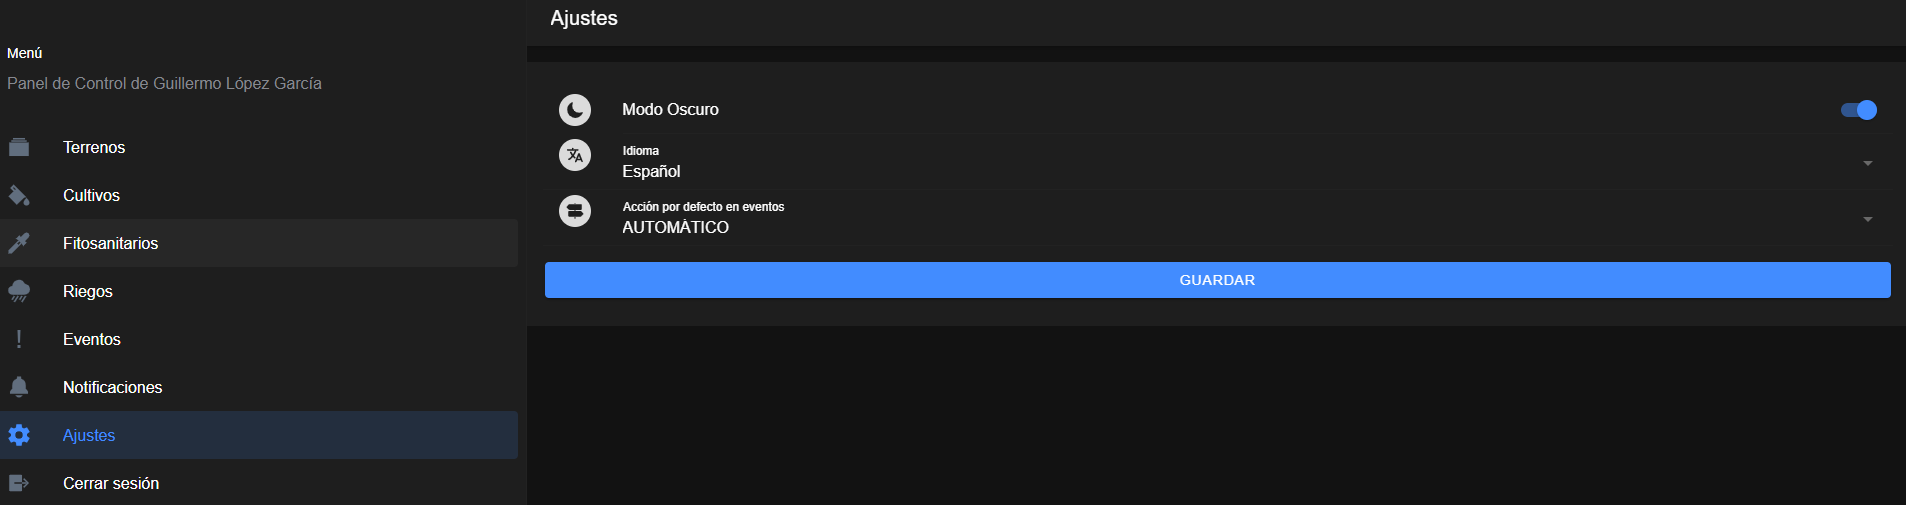
\includegraphics[width=0.7\linewidth]{images/user-manual/settings/update.png}
    \caption{Actualizar Ajustes}
\end{figure}